\section{Tutorial: PintaFotos}

En este tutorial presentaremos el componente \component{Lienzo} para
crear aplicaciones con gráficos y animaciones simples en 2 dimensiones
(2D). Construirás la aplicación \appName{PintaFotos} que permite al
usuario dibujar en la pantalla usando distintos colores, usando una
imagen de fondo y dibujando sobre ella.

\emph{Un dato histórico}: PintaFotos fue uno de los primeros programas
desarrollados para demostrar el potencial de los computadores, en la
decada de 1970. En aquel entonces, hacer algo tan simple como esta
aplicación de dibujo era algo muy complejo, y los resultados no eran
perfectos. Pero ahora, con \AppInventor, cualquiera puede rápidamente
armar una aplicación de dibujo bastante buena, lo que sirve de
excelente punto de partida para luego hacer juegos 2D.

La interfaz de usuario de \appName{PintaFotos} se muestra en
la~\Cref{fig:appUI}.

\begin{figure}[H]
\centering
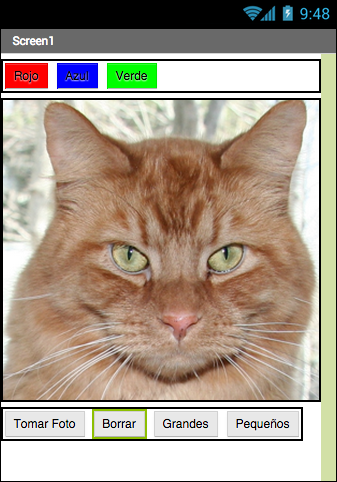
\includegraphics[scale=0.5]{PintaFotosUI}
\caption{Interfaz de usuario aplicación \appName{PintaFotos}}
\label{fig:appUI}
\end{figure}

En esta aplicación podrás:

\begin{itemize}
\item Bañar tu dedo en un tarro de pintura virtual para dibujar en
  este color.
\item Arrastrar tu dedo en la pantalla para dibujar una línea.
\item Tocar la pantalla para hacer puntos.
\item Usar el botón de abajo para limpiar la pantalla.
\item Agrandar o achicar el tamaño de los puntos con los botones
  abajo.
\item Sacar una foto con la cámara y luego dibujar encima de esta foto.
\end{itemize}

\subsection*{Qué Aprenderás}

Siguiendo este tutorial aprenderás a:

\begin{itemize}
\item Usar el componente \component{Lienzo} para dibujar.
\item Manejar las funcionalidades “touch” y “arrastrar” en la pantalla del equipo.
\item Configurar la disposición de los componentes en la pantalla.
\item Usar los controladores de eventos que reciben argumentos o
  parámetros.
\item Definir variables para recordar cosas como el tamaño de un punto
  elegido por el usuario para dibujar.
\end{itemize}

\subsection*{Para Empezar}

Asegúrate que tu computador y teléfono están configurados para usar
\AppInventor. Crea un nuevo proyecto y nómbralo \appName{PintaFotos}. Abre el
\blockEditor y comprueba que puedes probar tu aplicación en tu
dispositivo mediante la conexión USB. Consulta con tu tutor ante
cualquier problema!

Para empezar, ve al panel de propiedades a la derecha del \designer y
cambia el título de la pantalla a ``PintaFotos''. Deberías ver este
cambio reflejado en el teléfono, con el nuevo título apareciendo en la
barra de títulos de tu app.

Si estás preocupado por confundir el nombre de tu proyecto con el
nombre de la pantalla, no te preocupes! Hay tres nombres claves en
\AppInventor:

\begin{itemize}	

\item El nombre que eliges para tu proyecto mientras trabajes en
  él. También será el nombre de la aplicación cuando la quieras
  publicar. Nota que puedes hacer click en “Archivo” y seleccionar
  ``Guardar Como'' en el \designer para crear una nueva versión o
  cambiar el nombre de un proyecto.

\item El nombre de la componente, \component{Screen1}, que verás en el
  panel que contiene el listado de los componentes de la app. No
  puedes cambiar este nombre en esta versión de \AppInventor.

\item El título de la pantalla, él que ves en la barra de título del
  teléfono. Empieza siendo \component{Screen1}, que es el título que
  usaste en \appName{HolaGatito}. Pero lo puedes cambiar, como lo
  hicimos en \appName{PintaFotos}.
\end{itemize}

\subsection*{Diseñando los Componentes}

Para crear la app usarás los siguientes componentes:

\begin{itemize}

\item Tres componentes \component{Botón} para seleccionar pintura
  roja, azul o verde y un componente \component{DisposiciónHorizontal}
  para organizarlos.

\item Un componente \component{Botón} para limpiar el dibujo, y otros
  dos para cambiar el tamaño de los puntos.

\item Un componente \component{Lienzo}, que es la superficie para
  dibujar. El \component{Lienzo} tiene una propiedad
  \property{ImagenDeFondo}, que configuraremos como
  \mediafile{gatito.png} desde el tutorial \appName{Hola Gatito}. Más
  adelante, modificarás la app para que la imagen de fondo pueda ser
  una foto sacada por el usuario.

\end{itemize}

\subsubsection*{Crea los Botones de Colores}

Primero, crea los 3 botones de color usando las siguientes
instrucciones:

\begin{itemize}
\item Arrastra un \component{Botón} al \viewer y cambia su
  \property{Texto} a ``Rojo'', y su \property{ColorDeFondo} también a
  rojo.

\item En la lista de \componentList, selecciona el \component{Botón1}
  y presiona ``Cambiar Nombre'' para cambiar su nombre por
  \component{BotónRojo}. Observa que no se puede poner espacios en los
  nombres de los componentes, entonces es común poner en mayúscula la
  primera letra de cada palabra en el nombre.

\item De la misma manera, crea dos botones adicionales para azul y
  verde, nombrados \component{BotónAzul} y \component{BotónVerde}
  respectivamente. Ponlos debajo del botón rojo. Chequea tu trabajo
  comparándolo con la~\Cref{fig:PaintPot1}.

\end{itemize}

\begin{figure}[H]
\vspace{3em}
\centering
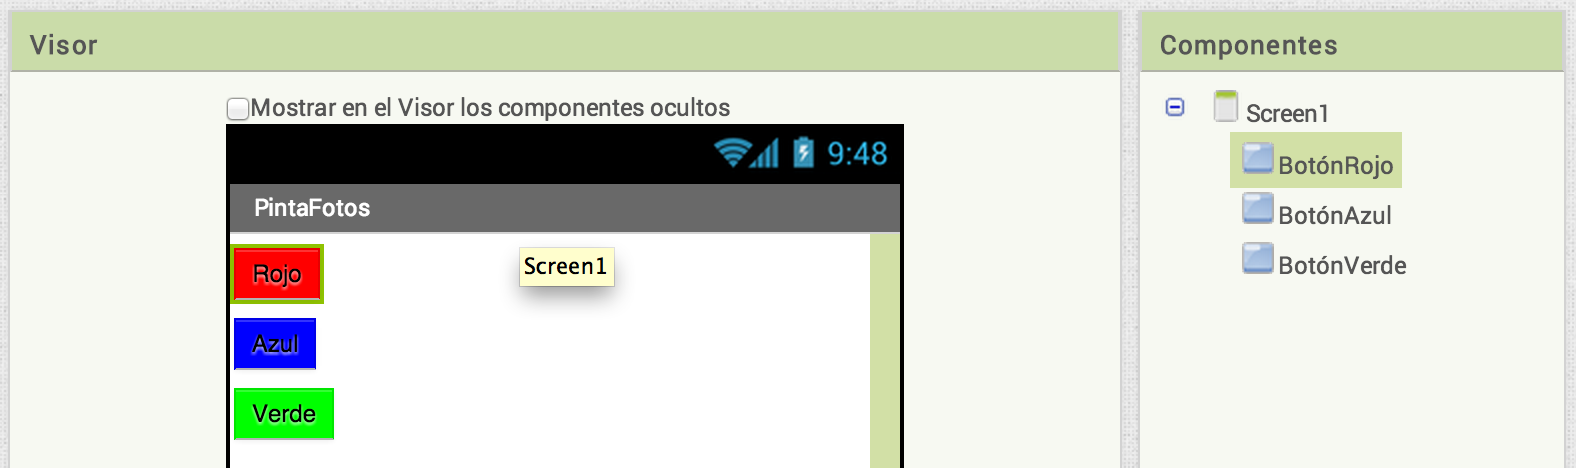
\includegraphics[scale=0.5]{PaintPot1}
\caption{El \viewer con los tres botones creados.}
\label{fig:PaintPot1}
\end{figure}

\paragraph{Importante!}
Observa que en este proyecto cambias los nombres de los componentes en
vez de dejarlos con sus nombres por defecto, como lo hiciste en
\appName{Hola Gatito}. El usar nombres más significativos hace que tus
proyectos sean más fáciles de leer, y realmente ayuda en el momento de
pasar al \blockEditor cuando tendrás que referirte a los componentes
por su nombre. A partir de ahora y en el resto del taller usaremos la
convención de que cada nombre de componente empiece por su tipo (por
ejemplo: \component{BotónRojo}).

\paragraph{Prueba tu aplicación!} Conecta tu aplicación a tu
dispositivo y verifica que funcione correctamente.

\subsubsection*{Usando los Componentes de Disposición para una Mejor
  Presentación}

Ahora deberías tener tres botones alineados verticalmente. Sin embargo
para esta app, vas a necesitar que estén en fila horizontal arriba de
la pantalla, como en la~\Cref{fig:PaintPot2}. Para ello debes usar el
componente \component{DisposiciónHorizontal}.

\begin{figure}[H]
\centering
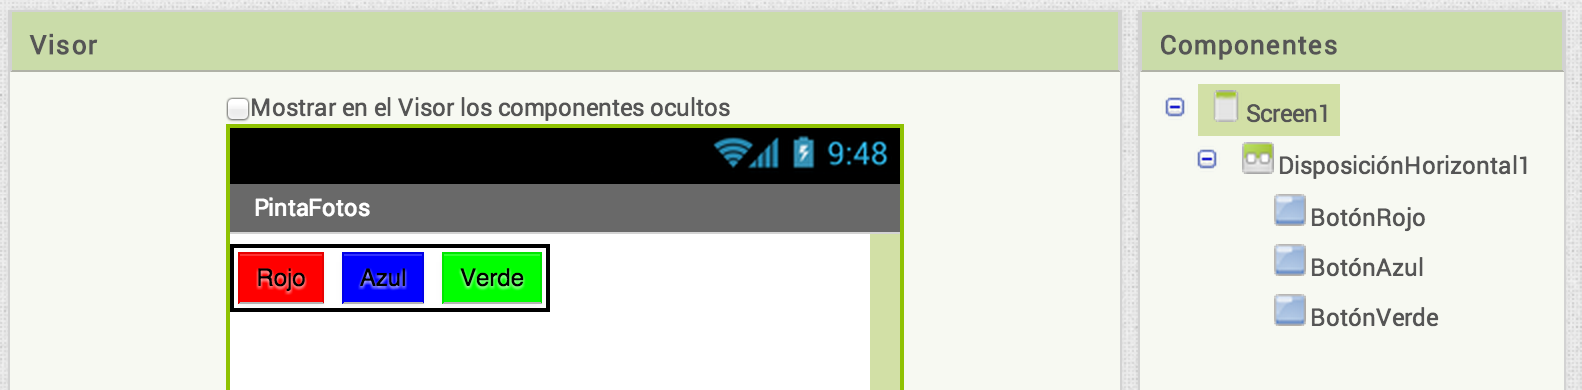
\includegraphics[scale=0.5]{PaintPot2}
\caption{Los tres botones en disposición horizontal.}
\label{fig:PaintPot2}
\end{figure}

\begin{enumerate}

\item Desde la categoría “Disposición'' en la \palette, arrastra un
  componente \component{DisposiciónHorizontal} y ponlo debajo de los
  botones.

\item En el panel de \properties, cambia el \property{Ancho} de
  \component{DisposiciónHorizontal} a la opción ``Ajustar al
  contenedor'' para llenar todo lo ancho de la pantalla.

\item Mueve los tres botones uno después del otro al interior de la
  \component{DisposiciónHorizontal}. \emph{Truco}: Verás una línea
  vertical azul que indica dónde irá el elemento que estás
  arrastrando.

\end{enumerate}

Si miras en la lista de componentes del proyecto, verás tres botones
listados bajo el componente \component{DisposiciónHorizontal}, lo que
muestra que se trata de sus subcomponentes. Asímismo, observa que
todos los componentes están listados bajo el componente
\component{Screen1}.

\paragraph{Prueba tu Aplicación!} Deberías ver tus tres botones en una
fila horizonal en la pantalla, a pesar de que puedan verse un poco
diferente a como se ven en el \designer. Por ejemplo, el borde de
\component{DisposiciónHorizontal} no aparece en el dispositivo.

En general, se usan los componentes de ``Disposición'' como opciones
de diseño para crear disposiciones simples, verticales, horizontales o
en tablas. También puedes crear disposiciones más complejas insertando
componentes de disposición unos dentro de otros.

\subsubsection*{Agregar el Lienzo}

\begin{itemize}

\item El lienzo es el lugar donde el usuario dibuja círculos y
  líneas. Agregalo, y configura el archivo \mediafile{gatito.png},
  usado en \appName{Hola Gatito}, como su \property{ImagenDeFondo}.

\item Desde la categoría ``Dibujo y Animación'' de la \palette,
  arrastra un \component{Lienzo} hacia el \viewer. Cambia su nombre a
  \component{LienzoDeDibujo}. Configura su \property{Ancho} como
  ``Ajustar al Contenedor'' y su \property{Alto} a 300 pixeles.

\item Recuerda que puedes descargar el archivo \mediafile{gatito.png}
  desde \resources{ProgramaTusIdeas/Dia1/HolaGatito}.

\item Configura la \property{ImagenDeFondo} del
  \component{LienzoDeDibujo} con el archivo \mediafile{gatito.png}. Si
  es necesario, debes subir el archivo.

\item Cambia el \property{ColorDePintura} en el
  \component{LienzoDeDibujo} al color rojo para que cuando
  el usuario inicie la app pero todavía no ha presionado ningun botón,
  sus dibujos sean rojos. Comprueba si lo que has hecho es parecido a
  la~\Cref{fig:PaintPot3}.

\begin{figure}[H]
\centering
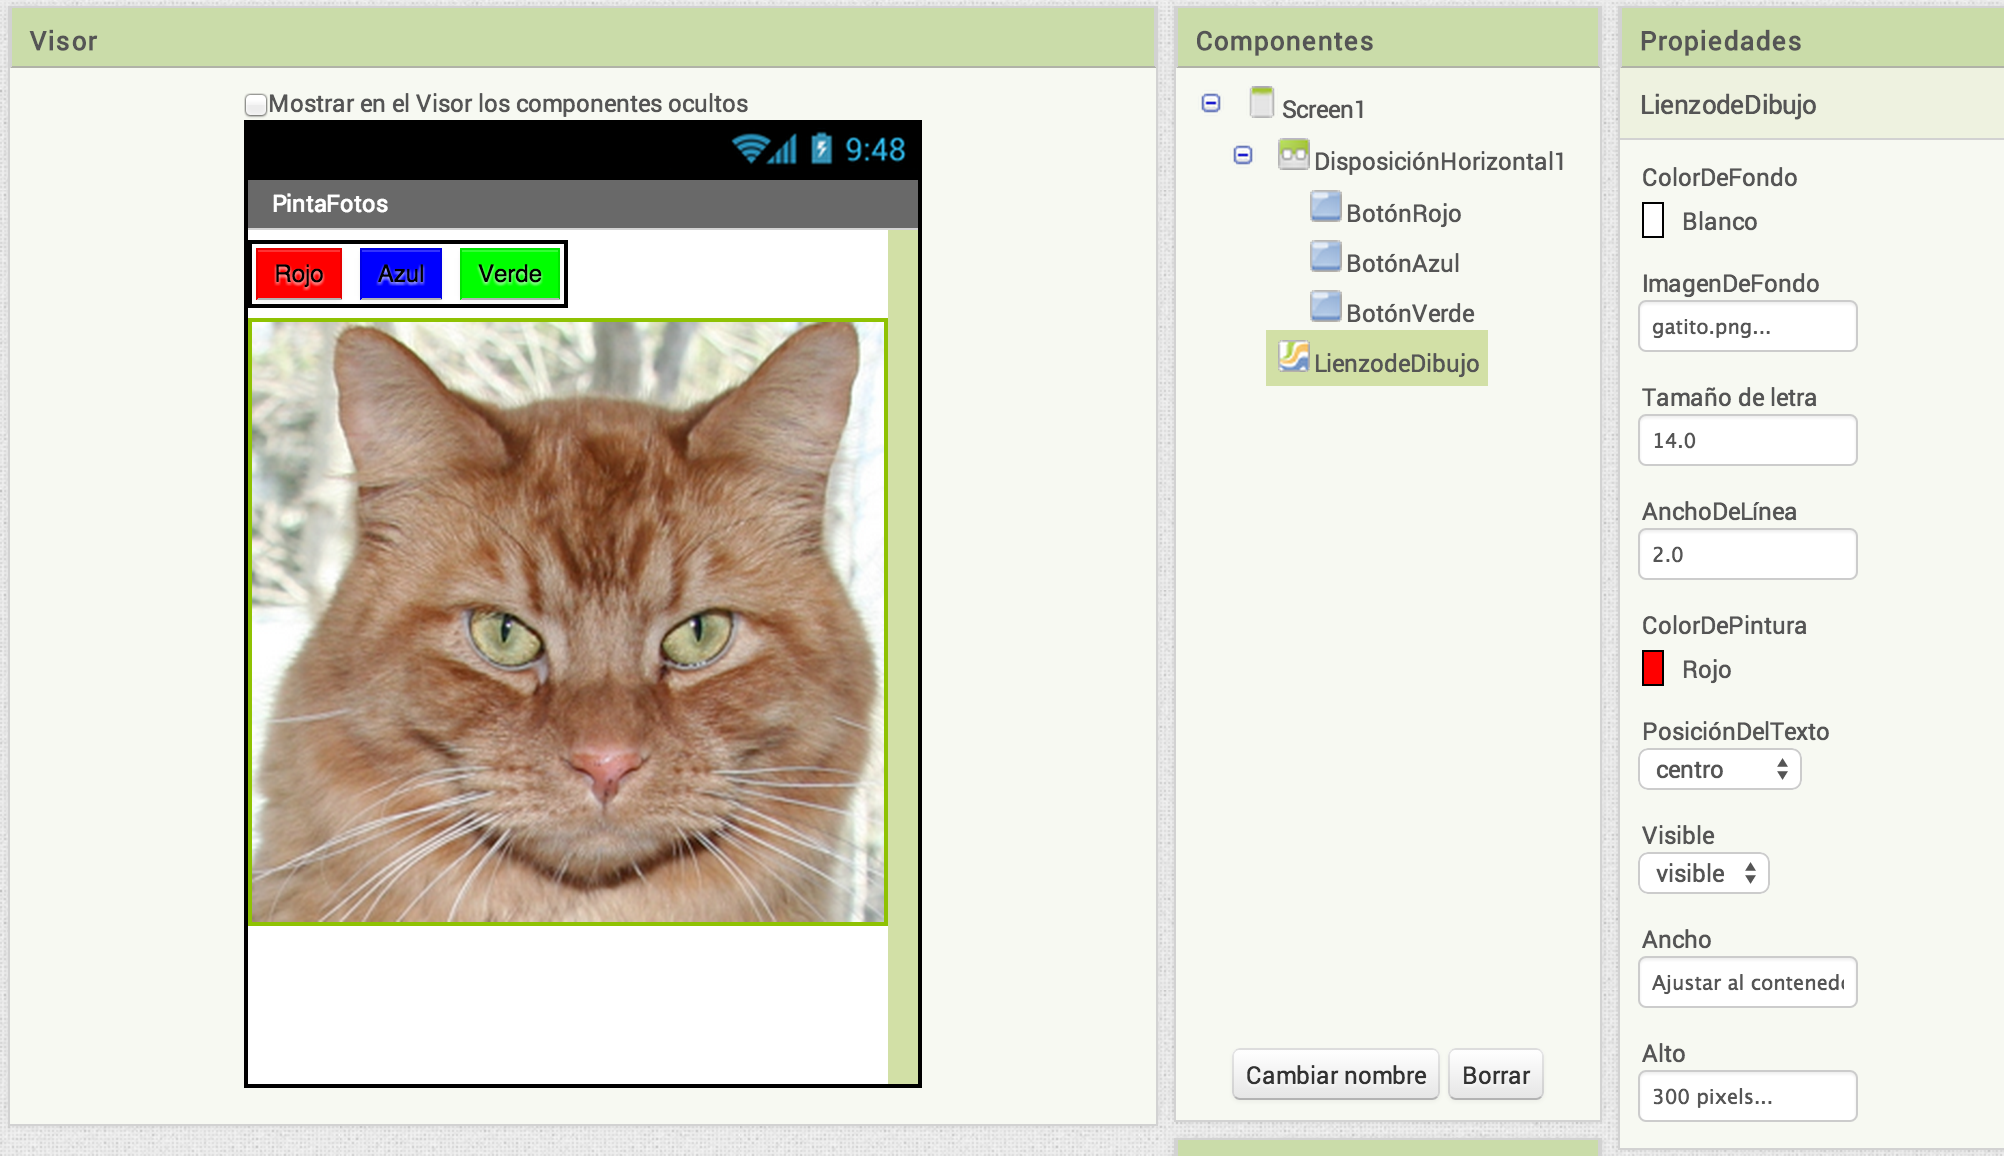
\includegraphics[scale=0.5]{PaintPot3}
\caption{El \component{LienzoDeDibujo} con la imagen
  \mediafile{gatito.png} como \property{ImagenDeFondo}.}
\label{fig:PaintPot3}
\end{figure}

\end{itemize}

\subsubsection*{Agregar los Botones Inferiores y el Componente Cámara}

\begin{enumerate}

\item Desde la \palette, arrastra un nuevo componente
  \component{DisposiciónHorizontal} y ponlo abajo del lienzo.

\item Luego arrastra dos componentes \component{Botón} adicionales en
  el \viewer y ponlos dentro del \component{DisposiciónHorizontal} que
  acabas de agregar. Cambia el nombre del primer botón por
  \component{BotónCámara} y su \property{Texto} a ``Sacar
  Foto''. Cambia el nombre del segundo botón por
  \component{BotónLimpiar} y su \property{Texto} por ``Limpiar''.

\item Arrastra dos botones más y colócalos al lado derecho del
  \component{BotónLimpiar}.

\item Nombra los nuevos botones como \component{BotónGrande} y
  \component{BotónPequeño}, y pon su \property{Texto} como
  ``Grande'' y ``Pequeño'' respectivamente.

\item Desde la sección \media de la \palette, arrastra un componente
  \component{Cámara} hacia el \viewer. Aparecerá en la sección de los
  componentes no-visibles.

\end{enumerate}
	
Una vez completados estos pasos, tu aplicación debería verse como en
la~\Cref{fig:PaintPot4}.

\begin{figure}[H]
\centering
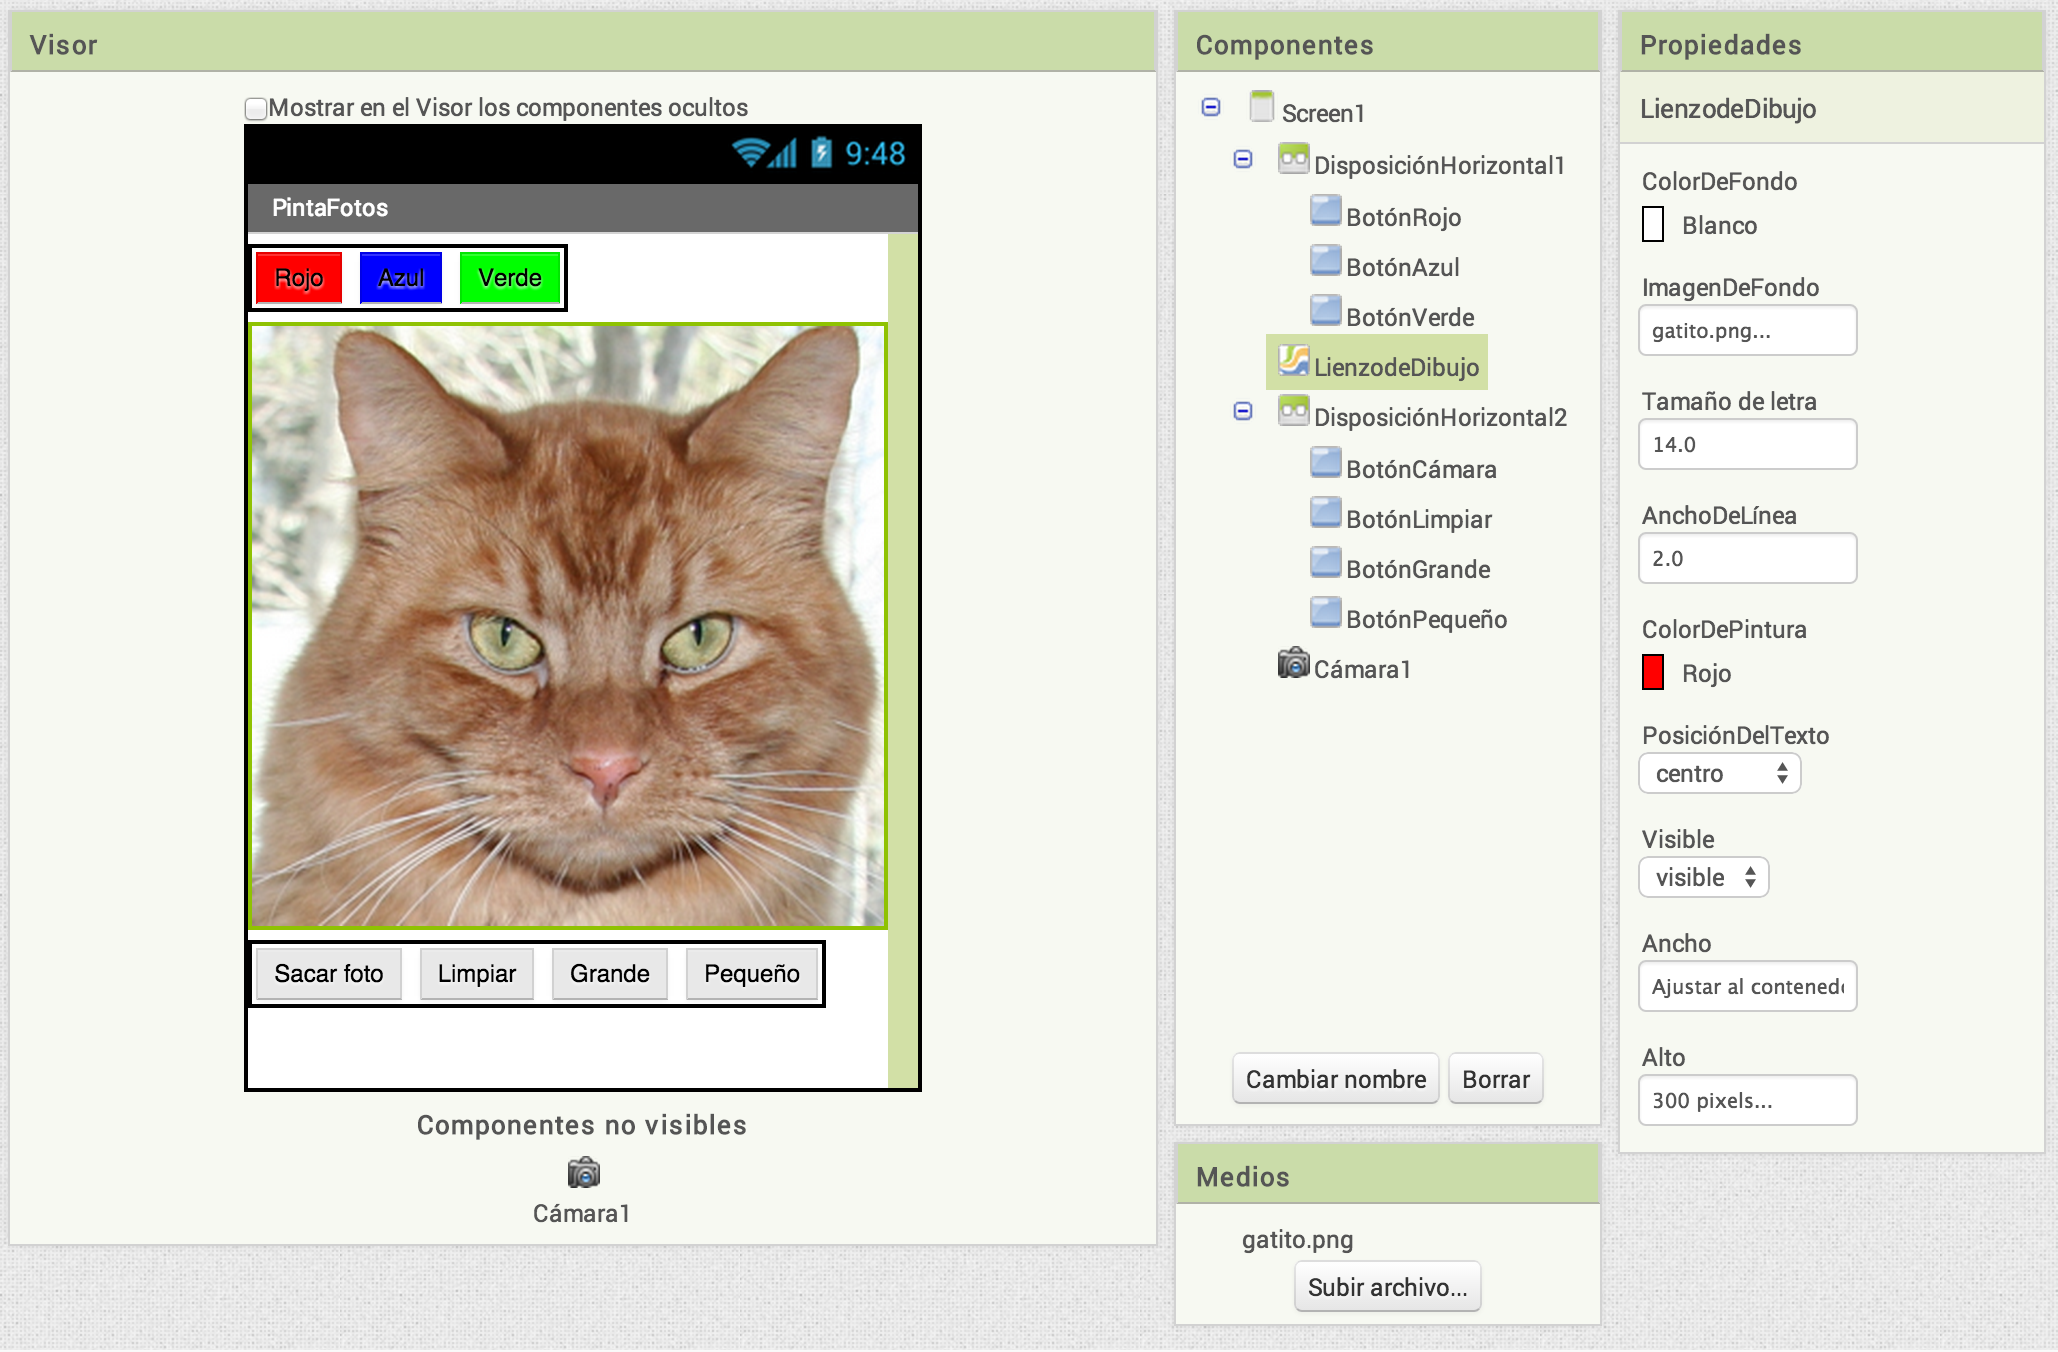
\includegraphics[scale=0.5]{PaintPot4}
\caption{Interfaz de usuario completa para \appName{PintaFotos}}
\label{fig:PaintPot4}
\end{figure}

\paragraph{Prueba tu Aplicación!} ¿Aparece la foto del gatito debajo
de los botones de la primera fila? ¿Aparece la última fila de botones abajo?

\subsubsection*{Agregar Comportamiento a los Componentes}

El próximo paso es definir cómo se comportan los componentes. Crear un
programa de pintura puede parecer un desafío insuperable, pero quedate
tranquilo! \AppInventor te facilita el trabajo: existen bloques muy
fáciles de usar para manejar las funcionalidades de touch y arrastre,
y para dibujar y sacar fotos.

En el \designer, agregaste un componente \component{Lienzo} llamado
\component{LienzoDeDibujo}. Como todos los componentes de ese tipo,
\component{LienzoDeDibujo} tiene un evento \block{Tocar} y un evento
\block{Arrastrado}. Programarás el evento \block{LienzoDibujo.Tocar}
de tal manera que llame a la función
\block{LienzoDibujo.DibujarCírculo}. Programarás el evento
\block{LienzoDibujo.Arrastrado} de tal manera que llame a la función
\block{LienzoDibujo.DibujarLínea}. Programarás luego los botones para
configurar la propiedad \property{ColorDePintura} usando el bloque
\block{poner LienzoDibujo.ColorPintura}, y para limpiar el
\component{LienzoDeDibujo}; y finalmente, programarás como cambiar la
\property{ImagenDeFondo} del lienzo por una foto sacada con la cámara
del dispositivo.

\subsubsection*{Agregar el Evento Tocar para Dibujar un Punto}

Primero, dispondrás los objetos de manera que cuando tocas el
\component{LienzoDeDibujo}, se dibuje un punto en el lugar del lienzo que
toques:
	
\begin{enumerate}

\item En el \blockEditor, selecciona el \component{LienzoDeDibujo}, y
  arrastra el bloque \block{LienzoDeDibujo.Tocado} al \viewer. El
  bloque tiene parámetros para \parameter{x} e \parameter{y},
  y \parameter{SpriteTocado}, como ilustrado en
  la~\Cref{fig:PaintPot5}. Estos parámetros entregan información sobre
  la ubicación del evento ``tocar la pantalla'' hecho por el usuario.

\begin{figure}[H]
\centering
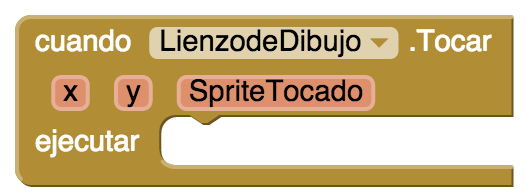
\includegraphics[scale=0.5]{PaintPot5}
\caption{El evento viene con información sobre la ubicación del toque
  en la pantalla}
\label{fig:PaintPot5}
\end{figure}

\textbf{Nota}. Si completaste la aplicación \appName{Hola Gatito}, ya
estás familiarizado con los eventos de \block{Botón.Click}, pero no
con los eventos del lienzo. Los eventos \block{Botón.Click} son
bastante sencillos porque no hay nada más que saber del evento aparte
del hecho que ocurrió. Algunos controladores de eventos, sin embargo,
vienen con información sobre los argumentos para llamar al evento. El
evento \block{LienzoDibujo.Tocar} te entrega las
coordenadas \parameter{x} e \parameter{y} del toque dentro del
\component{LienzoDeDibujo}. También te dice si un objeto dentro del
\component{LienzoDeDibujo} (lo que se conoce como \emph{Sprite}) fue
tocado, pero este punto se abordará más adelante. Las
coordenadas \parameter{x} e \parameter{y} son los argumentos que
usaremos para grabar dónde el usuario tocó la pantalla, de manera de
poder dibujar el punto en este lugar.

\item Arrastra un bloque \block{LienzoDeDibujo.DibujarCírculo} desde
  el bloque y ponlo dentro del controlador de eventos
  \block{LienzoDeDibujo.Tocar}, como se ilustra en
  la~\Cref{fig:PaintPot6}.

\begin{figure}[H]
\centering
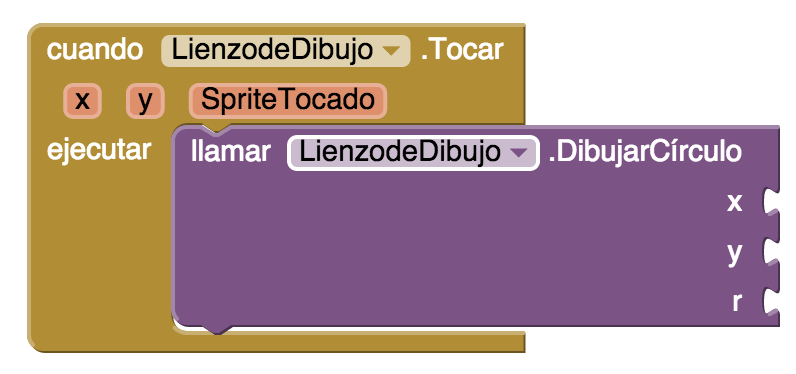
\includegraphics[scale=0.5]{PaintPot6}
\caption{Cuando el usuario toca el lienzo, la aplicación dibuja un círculo}
\label{fig:PaintPot6}
\end{figure}

Por el lado derecho del bloque
\component{LienzoDeDibujo.DibujaCírculo}, verás tres espacios vacíos
por completar con los argumentos
siguientes: \parameter{x}, \parameter{y},
y \parameter{r}. Los \parameter{x} e \parameter{y} especifican la
ubicación donde el círculo se va a dibujar, y \parameter{r} determina
el radio (o tamaño) del círculo.

El signo amarillo con el punto de exclamación a la izquierda inferior
de la pantalla aparecerá con un 1 cuando un espacio todavía permanece
vacío. Construiremos los bloques para completar esto después.

Este controlador de evento puede confundir un poco porque el evento
\block{LienzoDeDibujo.Tocar} también tiene una \parameter{x} y
una \parameter{y}. Solamente acuérdate que la \parameter{x} y
la \parameter{y} para el evento \block{LienzoDeDibujo.Tocar} te dice
dónde tocó el usuario, mientras que el \parameter{x} e \parameter{y}
para el evento \block{LienzoDeDibujo.DibujarCírculo} son espacios
abiertos para que tú definas donde se dibujará el círculo. Dado que
quieres que el círculo aparezca donde tocó el usuario, conectarás los
valores \parameter{x} e \parameter{y} desde el
\block{LienzoDeDibujo.Tocar} de la misma forma que los valores de los
parámetros \parameter{x} e \parameter{y} en
\block{LienzoDeDibujo.DibujarCírculo}.

Nota. Puedes acceder a los valores del evento al pasar el mouse sobre
los parámetros en el bloque ``Cuando''. Al hacerlo, aparecerán los
bloques \block{tomar} y \block{poner a}. Arrastra el bloque
\block{tomar x} y conéctalo como el valor faltante en
para \parameter{x} en \block{LienzoDeDibujo.DibujarCírculo}, como se
ilustra en la~\Cref{fig:PaintPot7}.

\begin{figure}[H]
\centering
\vspace{3em}
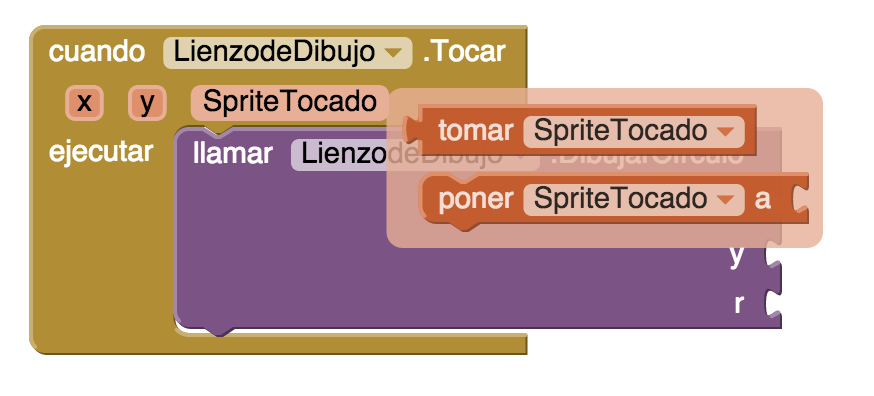
\includegraphics[scale=0.5]{PaintPot7}
\caption{Para acceder al parámetro de un evento, arrastra un bloque
  \block{tomar} desde el bloque \block{LienzoDeDibujo.Tocar}}
\label{fig:PaintPot7}
\end{figure}

\item Arrastra los bloques \block{tomar x} y \block{tomar y} y
  conéctalos en los espacios abiertos en el bloque
  \block{LienzoDeDibujo.DibujarCírculo}, como se ilustra en
  la~\Cref{fig:PaintPot8}.

\begin{figure}[H]
\centering
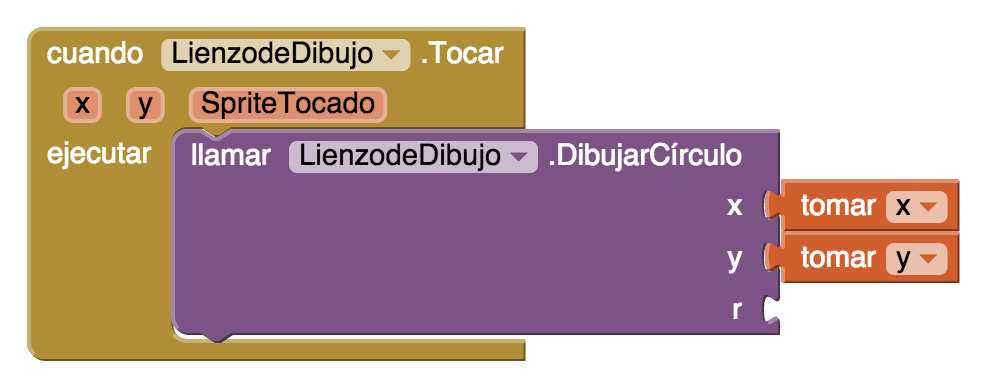
\includegraphics[scale=0.5]{PaintPot8}
\caption{La aplicación sabe donde dibujar (x,y), pero todavía necesitamos
  especificar cuán grande debería ser el círculo.}
\label{fig:PaintPot8}
\end{figure}

\item Ahora necesitas especificar el radio del círculo a dibujar. El
  radio se mide en \emph{pixeles}, que es el punto más pequeño que
  puede ser dibujado en la pantalla. Por ahora, ponle como valor el
  número 5: haz click en una zona blanca de la pantalla y tipea 5,
  luego presiona Enter para crear automáticamente un bloque numérico,
  y conecta este bloque en el espacio para el
  parámetro \parameter{r}. Cuando hagas esto, el signo amarillo en la
  esquina inferior se pondrá en 0 nuevamente, dado que todos los
  espacios abiertos habrán sido completados. La~\Cref{fig:PaintPot9}
  muestra como debiera verse el controlador de eventos
  \block{LienzoDeDibujo.Tocar}.

\begin{figure}[H]
\vspace{3em}
\centering
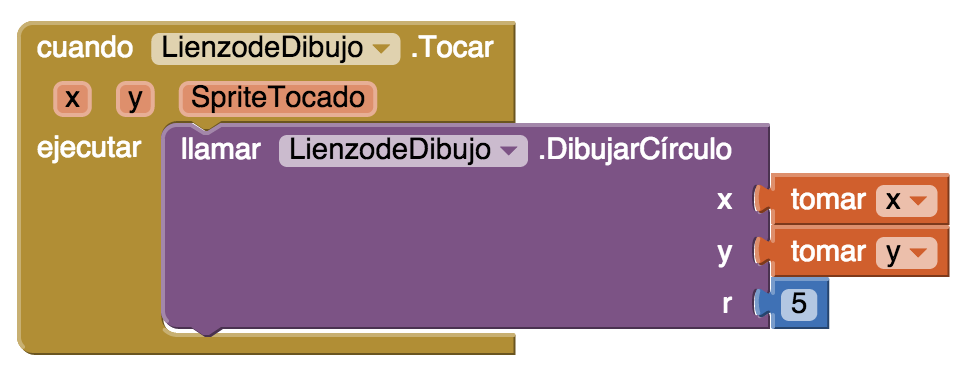
\includegraphics[scale=0.5]{PaintPot9}
\caption{Cuando el usuario toca el \component{LienzoDeDibujo}, un
  círculo de radio 5 será dibujado en las coordenadas (x, y)
  correspondientes.}
\label{fig:PaintPot9}
\end{figure}

  \textbf{Nota}. Al poner un 5 en el \blockEditor y luego presionar
  Enter, habrás usado lo que se llama \emph{tipeo de bloques}. Si
  empiezas a tipear, el editor de bloques muestra un listado de
  bloques cuyos nombres corresponden a lo que estás tipeando. Si
  tipeas un número, crea un bloque numérico.

  \paragraph{Prueba tu Aplicación!} Usa tu dispositivo para probar lo
  que has desarrollado hasta ahora. Al tocar el
  \component{LienzoDeDibujo}, tu dedo debería dejar un punto en cada
  lugar que toques. Los puntos serán rojos si configuraste la
  propiedad del \property{LienzoDeDibujo.ColorDePintura} como color
  rojo en el \designer (sino será negro, que es el color por defecto).

\end{enumerate}

\subsubsection*{Agregar el Evento de Arrastre para Dibujar una Línea}

Luego, agregarás el controlador de eventos de arrastre. La diferencia
entre un touch y un arrastre es la siguiente:
	
\begin{itemize}
\item Un touch es cuando pones tu dedo en la pantalla y solo lo
  levantas para tocar, sin desplazarlo.

\item Un arrastre es cuando pones tu dedo en la pantalla y lo mueves
  al mantener contacto con la pantalla.
\end{itemize}
	
En un programa de pintura, cuando arrastras tu dedo en la pantalla se
dibuja una línea igual al camino que sigue tu dedo. Lo que estás
haciendo en realidad es dibujar cientos de pequeñas líneas rectas;
cada vez que mueves tu dedo, incluso un poco, extiendes la línea desde
la última posición de tu dedo hacia su nueva posición.

\begin{enumerate}
	
\item En el \blockEditor, desde la sección del
  \component{LienzoDeDibujo}, arrastra el bloque
  \block{LienzoDeDibujo.Arrastrado} al espacio de trabajo. Deberías
  ver el gestionador de eventos tal como en la~\Cref{fig:PaintPot10}.

\begin{figure}[H]
\centering
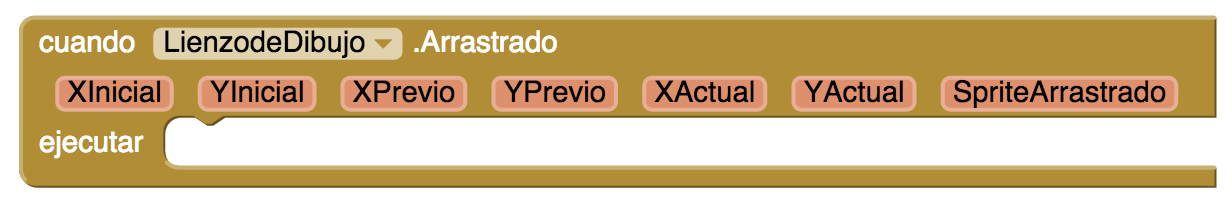
\includegraphics[scale=0.5]{PaintPot10}
\caption{Un evento de arrastre tiene más argumentos que un evento de touch.}
\label{fig:PaintPot10}
\end{figure}

El evento LienzoDibujo.Arrastre viene con los siguientes argumentos:

\begin{itemize}

\item \parameter{XInicial}, \parameter{YInicial}: la posición de tu
  dedo donde empieza el arrastre.

\item \parameter{XActual}, \parameter{YActual}: la posición actual de
  tu dedo.

\item \parameter{XPrevio}, \parameter{YPrevio}: la posición
  inmediatamente anterior de tu dedo.

\item \parameter{SpriteArrastrado}: un booleano, será verdad si el
  usuario hace el arrastre directamente sobre un imagen Sprite. En el
  taller no usaremos este argumento.

\end{itemize}

\item Arrastra el bloque \block{LienzoDeDibujo.DibujarLínea} dentro
  del bloque \block{LienzoDeDibujo.Arrastrado} como se muestra en
  la~\Cref{fig:PaintPot11}.

\begin{figure}[H]
\centering
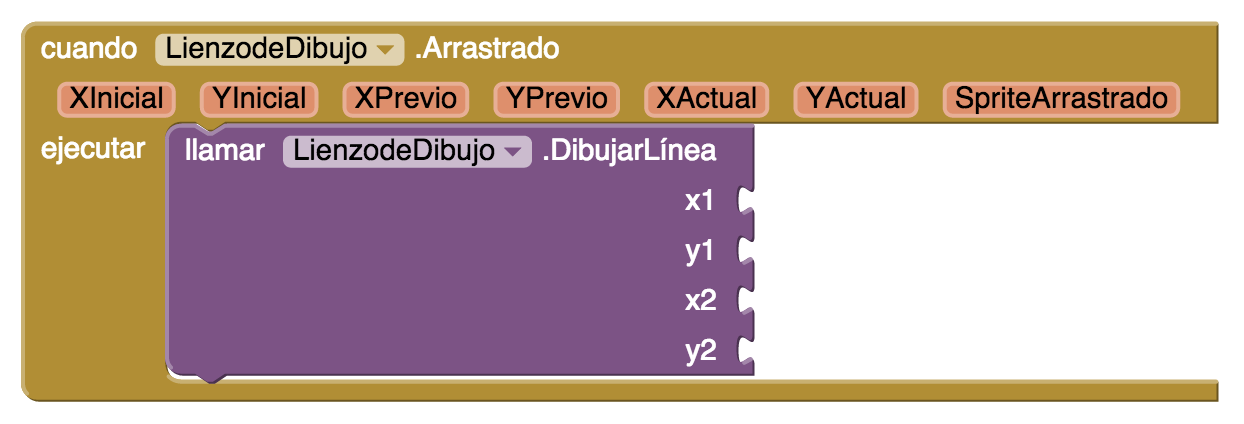
\includegraphics[scale=0.5]{PaintPot11}
\caption{Agregando la habilidad de dibujar líneas}
\label{fig:PaintPot11}
\end{figure}

El bloque \block{LienzoDeDibujo.DibujarLínea} tiene cuatro argumentos,
dos para cada punto que determina la línea: un punto es
(\parameter{x1}, \parameter{y1}), mientras que
(\parameter{x2}, \parameter{y2}) es el otro. ¿Puedes adivinar qué
valores corresponden a cada argumento?  Recuerda que el evento
\block{LienzoDeDibujo.Arrastrado} se activará cada vez que arrastres
tu dedo en el \viewer, por lo tanto la aplicación dibuja una pequeña
línea cada vez que mueves tu dedo, desde
(\parameter{XPrevio}, \parameter{YPrevio}) hacia
(\parameter{XActual}, \parameter{YActual}). Agreguemos esto a nuestro
bloque \block{LienzoDeDibujo.DibujarLínea}:

\item Arrastra los bloques \block{tomar} para los argumentos que vas a
  necesitar. Los valores \parameter{XPrevio} e \parameter{YPrevio}
  deberían ir conectados en los espacios para los
  argumentos \parameter{x1} e \parameter{y1}, respectivamente, como se
  ilustra en la~\Cref{fig:PaintPot12}.

\begin{figure}[H]
\centering
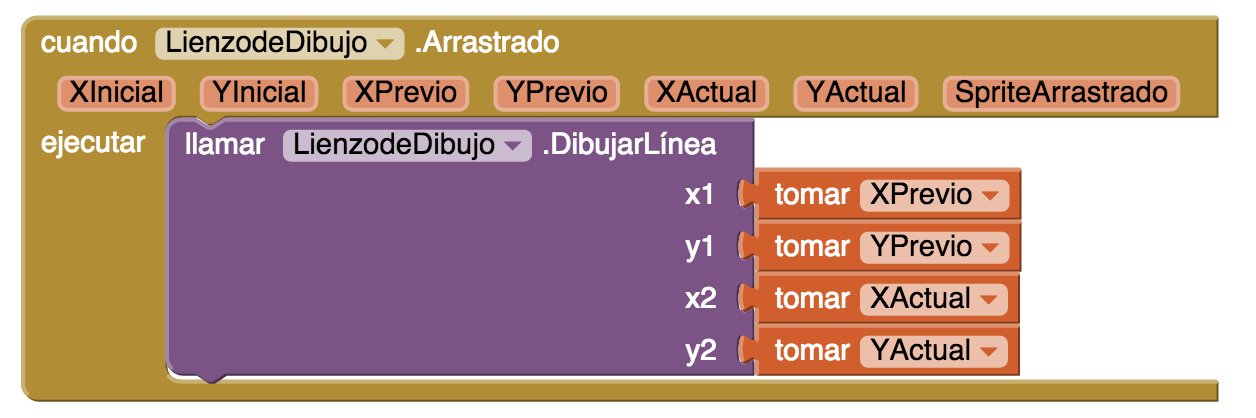
\includegraphics[scale=0.5]{PaintPot12}
\caption{Cuando el usuario arrastre el dedo, la aplicación dibujará
  una línea desde el punto anterior hacia el actual.}
\label{fig:PaintPot12}
\end{figure}

\paragraph{Prueba tu Aplicación!} Arrastra tu dedo en la pantalla para
dibujar líneas y curvas. Toca la pantalla para dibujar puntos.

\end{enumerate}

\subsubsection*{Agregar Controladores de Eventos para Botones}

La aplicación que has construido hasta ahora permite al usuario
dibujar, pero siempre estos dibujos usan el color rojo. El próximo
paso consiste en agregar controladores de eventos para los botones de
colores, para que el usuario pueda cambiar el color de la pintura, y
otro para el \component{BotónLimpiar} para que pueda limpiar la
pantalla y así volver a empezar a dibujar.

En el \blockEditor:

\begin{enumerate}
\item Arrastra el bloque \block{BotónRojo.Click} al espacio de
  trabajo.

\item Arrastra el bloque \block{poner LienzoDeDibujo.ColorDePintura} y
  conéctalo en las acciones del bloque \block{BotónRojo.Click}.

\item Abre la sección ``Colores'' y arrastra el bloque de color rojo
  para conectarlo con el bloque \block{poner
    LienzoDeDibujo.ColorDePintura}.

\item Repite los pasos anteriores para los botones azul y verde.

\item El último botón por configurar es el
  \component{BotónLimpiar}. Para limpiar el lienzo de dibujo debes
  utilizar el bloque \block{LienzoDeDibujo.Limpiar}. Confirma que tus
  bloques se ven como en la~\Cref{fig:PaintPot13}.

\begin{figure}[H]
\centering
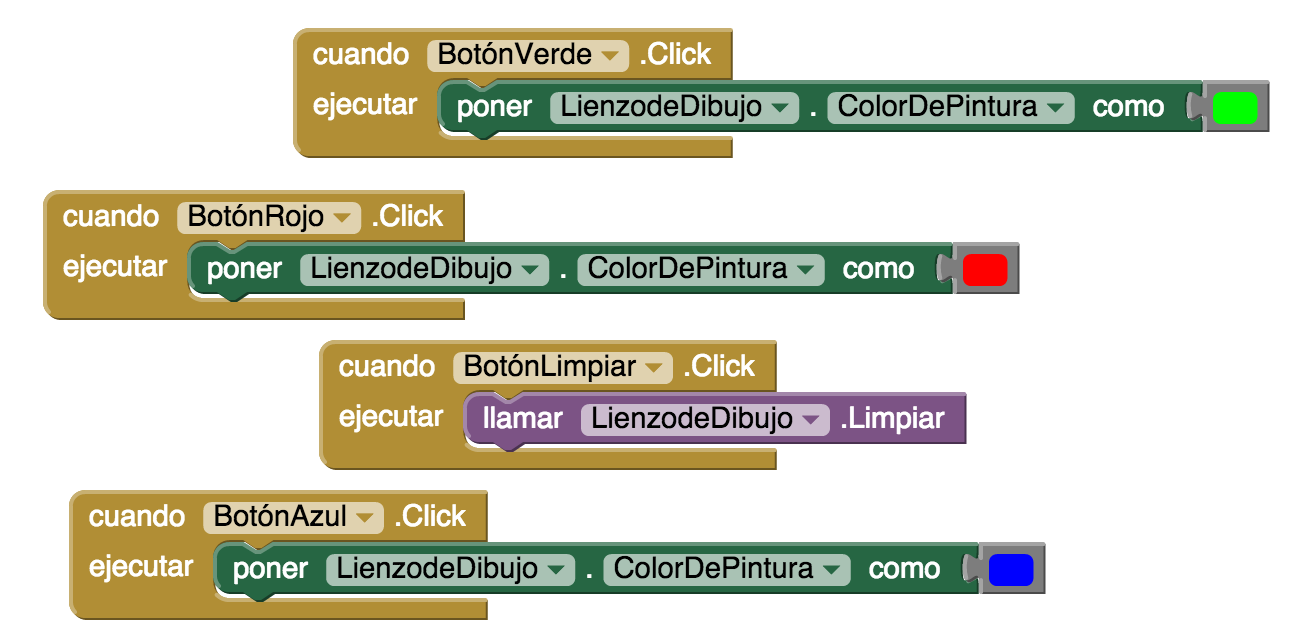
\includegraphics[scale=0.5]{PaintPot13}
\caption{Cuando el usuario hace click en los botones de colores cambia
el color para dibujar en el lienzo. Hacer click en ``Limpiar'', borra
el contenido del lienzo.}
\label{fig:PaintPot13}
\end{figure}

\end{enumerate}

\subsubsection*{Permitir al Usuario Tomar un Foto}

Las aplicaciones hechas con \AppInventor pueden interactuar con las
funcionalidades de los dispositivos Android, incluyendo la
cámara. Para personalizar la aplicación, se permite al usuario fijar
la imagen de fondo de su dibujo con una foto tomada con la cámara.

\begin{enumerate}

\item El componente \component{Cámara} contiene dos bloques claves. El
  bloque \block{Cámara.TomarFoto} inicia la aplicación de cámara del
  teléfono. El evento \block{Cámara.DespuésDeTomarFoto} se activa
  cuando el usuario terminó de sacar la foto. Agregarás bloques en el
  controlador de eventos \block{Cámara.DespuésDeTomarFoto} para
  configurar el \block{LienzoDeDibujo.ImagenDeFondo} con la foto que
  fue sacada. Abre la sección de \component{BotónCámara} y arrastra el
  controlador de evento \component{BotónCámara.Click} hacia el espacio
  de trabajo.

\item Arrastra el bloque \block{Cámara1.TomarFoto} y ponlo en el
  controlador \block{BotónCámara.TomarFoto}.

\item Arrastra el controlador de eventos
  \block{Cámara1.DespuésDeTomarFoto} al espacio de trabajo.

\item Arrastra el bloque \block{poner LienzoDeDibujo.ImagenDeFondo} y
  ponlo en las acciones de \block{Cámara1.DespuésDeTomarFoto}.

\item \block{Cámara1.DespuésDeTomarFoto} tiene un argumento
  llamado \parameter{imagen}, que es la foto recién sacada. Puedes
  referirte a ella, con un bloque ``tomar'' desde el bloque
  \block{Cámara1.DespuésDeTomarFoto}. Conecta la imágen como el
  argumento para el bloque \block{poner LienzoDeDibujo.ImagenDeFondo}.
	
  Los bloques deberían ser parecidos a la~\Cref{fig:PaintPot14}.

\begin{figure}[H]
\centering
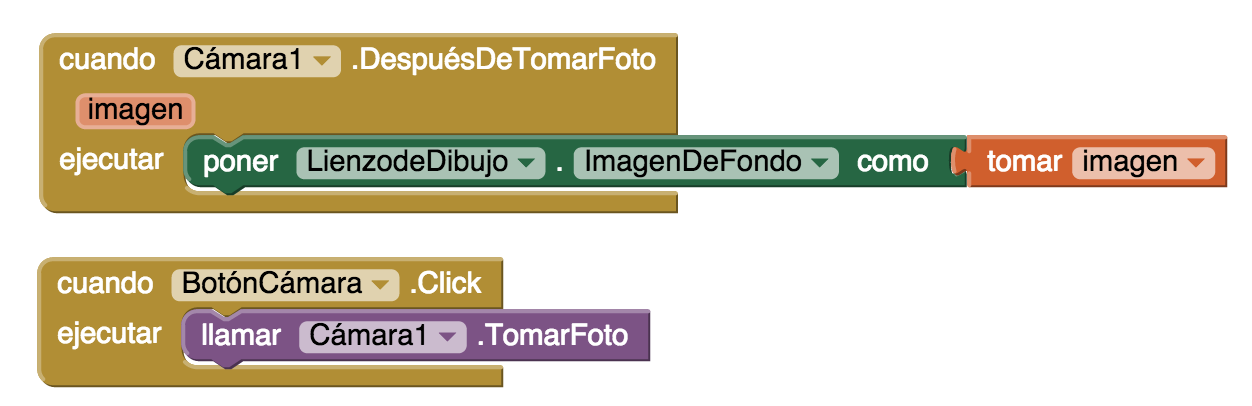
\includegraphics[scale=0.5]{PaintPot14}
\caption{CUando se saca la foto, se configura como la imagen de fondo
  del lienzo.}
\label{fig:PaintPot14}
\end{figure}

\paragraph{Prueba tu Aplicación!} Haz una prueba al hacer click en
``Tomar Foto'' y saca una foto. El gatito debería cambiar por la foto
que acabas de sacar, y luego podrás dibujar encima de la foto que
sacaste.

\end{enumerate}

\subsubsection*{Cambiar el Tamaño del Punto}

El tamaño de los puntos dibujados en el \component{LienzoDeDibujo} se
determina al llamar a \block{LienzoDeDibujo.DibujarCírculo}, donde el
argumento de radio está configurado en 5. Para cambiar el grueso de la
línea, puedes cambiar el valor de \parameter{r}. Para probar esto,
intenta cambiar el 5 por un 10 y pruébalo en el teléfono para ver cómo
aparece.

El único tamaño que el usuario podrá usar es el que tú indicas como
argumento para el radio del círculo. ¿Pero qué pasa si el usuario
quiere cambiar el tamaño de los puntos? Vamos a modificar el programa
de manera que el usuario---no solo el programador---pueda cambiar el
tamaño de los puntos. Lo haremos de tal manera que cuando el usuario
haga click en un botón llamado ``Grandes'', el tamaño será 8, y cuando
hará click en un botón llamado ``Pequeños'', será 2.

Para usar distintos valores en el argumento radio, la aplicación
necesita saber cuál queremos aplicar. Necesitamos pedirle usar un
valor específico, y tiene que memorizar este valor de manera a poder
seguir usándolo. Cuando tu aplicación necesita guardar algo en memoria
que no sea una propiedad, puedes definir una \emph{variable}. Una
variable es una \emph{celda de memoria}. Es como un balde donde puedes
almacenar datos variables, como el tamaño del punto.

Empezamos por definir una variable \variable{TamañoPunto}:

\begin{enumerate}

\item En el \blockEditor, desde la sección ``Variables'', arrastra un
  bloque \block{Inicializar global nombre}. Cambia el texto
  ``nombre'' por ``TamañoPunto''.

\item Fíjate que el bloque \block{Inicializar global TamañoPunto}
  tiene un espacio abierto. Ahí es donde puede especificar el valor
  inicial de la variable, o su valor por defecto al iniciar la
  aplicación. Para esta aplicación, inicializa el
  \variable{TamañoPunto} en 2 creando un bloque con el número 2, y
  conectándolo en \block{Inicializar global TamañoPunto} como se
  ilustra en la~\Cref{fig:PaintPot15}.
\end{enumerate}

\begin{figure}[H]
\centering
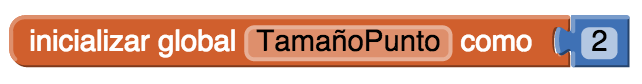
\includegraphics[scale=0.5]{PaintPot15}
\caption{Inicializar variable global \variable{TamañoPunto} con valor 2.}
\label{fig:PaintPot15}
\end{figure}

\subsubsection*{Usar las Variables}

Ahora, queremos cambiar el argumento de
\block{LienzoDeDibujo.DibujarCírculo} en el controlador de eventos
\block{LienzoDibujo.Tocar} para que uses el valor
\variable{TamañoPunto} en vez de usar siempre un número fijo. (Puede
dar la ilusión que fijamos \variable{TamañoPunto} en 2 porque lo
inicializamos de esta manera, pero verás en un minuto como podemos
cambiar \variable{TamañoPunto} y asi cambiar el tamaño del punto que
se dibuja.)

\begin{enumerate}
\item Arrastra un bloque ``tomar'' desde
  \block{LienzoDeDibujo.DibujarCírculo}. Deberías ver un bloque
  \block{tomar global TamañoPunto} que indica el valor de la variable.

\item Anda al controlador de eventos \block{LienzoDeDibujo.Tocar} y
  arrastra el bloque del número 5 fuera del espacio \parameter{r} y
  pónlo en el papelero.  Luego reemplázalo con el bloque \block{tomar
    global TamañoPunto} (Ver~\Cref{fig:PaintPot16}). Cuando el usuario
  toca el lienzo, la aplicación determinará ahora el radio a partir de
  la variable \variable{TamañoPunto}.
\end{enumerate}

\begin{figure}[H]
\vspace{3em}
\centering
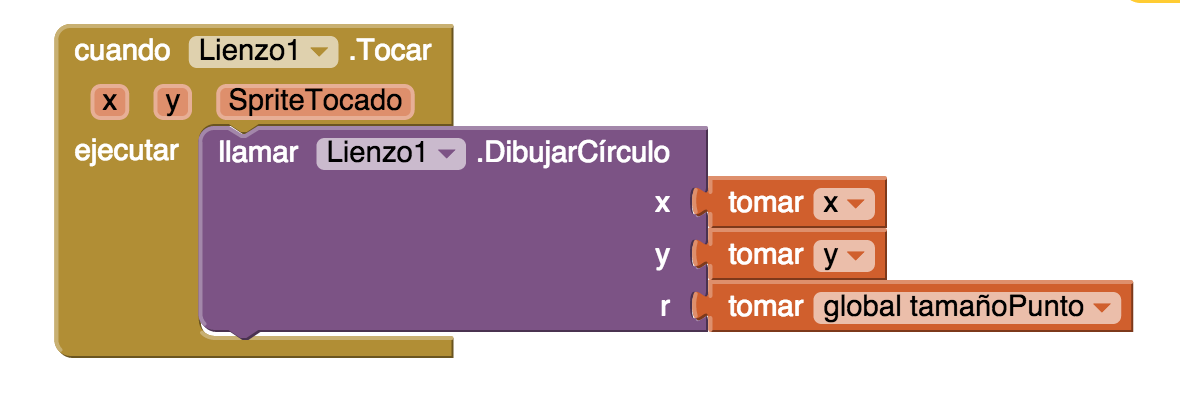
\includegraphics[scale=0.5]{PaintPot16}
\caption{Ahora el tamaño de cada círculo depende de lo
que está guardado en la memoria de la variable TamañoPunto.}
\label{fig:PaintPot16}
\end{figure}

\subsubsection*{Cambiar los valores de las variables}

Aquí es donde la magia de las variables opera. La variable
\variable{TamañoPunto} permite al usuario elegir el tamaño del
círculo, y tu controlador de eventos dibujará el círculo en función de
esto.  Desarrollaremos el comportamiento al programar los
controladores de eventos \block{BotónPequeño.Click} y
\block{BotónGrande.Click}.

\begin{enumerate}

\item Arrastra un controlador de eventos \block{BotónPequeño.Click}
    al espacio de trabajo. Luego arrastra desde la categoría
    ``Variables'' un bloque \block{poner a}, selecciona ``global
    TamañoPunto'' como referencia y conectalo a
    \block{BotónPequeño.Click}. Finalmente, crea un bloque número 2 y
    conéctalo al bloque \block{poner global TamañoPunto}.

\item Haz un controlador de eventos similar para
  \block{BotónGrande.Click}, pero configura el \variable{TamañoPunto} en 8. Ambos gestionadores de eventos
  deberían aparecer en el editor de bloques, como en la~\Cref{fig:PaintPot17}.

\end{enumerate}

\begin{figure}[H]
\centering
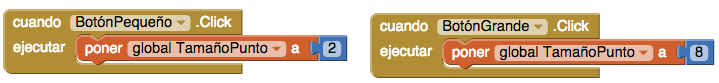
\includegraphics[scale=0.5]{PaintPot17}
\caption{Hacer click en los botones cambia el tamaño del
punto. Los toques que siguen serán con este tamaño de punto.}
\label{fig:PaintPot17}
\end{figure}

\paragraph{Prueba tu Aplicación!} Intenta hacer click en los botones
de tamaño y luego toca el lienzo. ¿Se dibujan círculos de distintos
tamaños? ¿Las líneas? El tamaño de las líneas no debería cambiar
porque programaste \variable{TamañoPunto} solamente para ser usado en
el bloque de \block{DibujarCírculo}. En base a esto, ¿podrías ahora
cambiar tus bloques para que el usuario también pueda cambiar el
tamaño de la línea? (Nota que el lienzo tiene una propiedad llamada
\property{AnchodeLinea})

\subsubsection*{La App Completa: PintaFotos}

La~\Cref{fig:PaintPot18} ilustra el código completo de la aplicación \appName{PintaFotos}:

\begin{figure}[H]
\centering
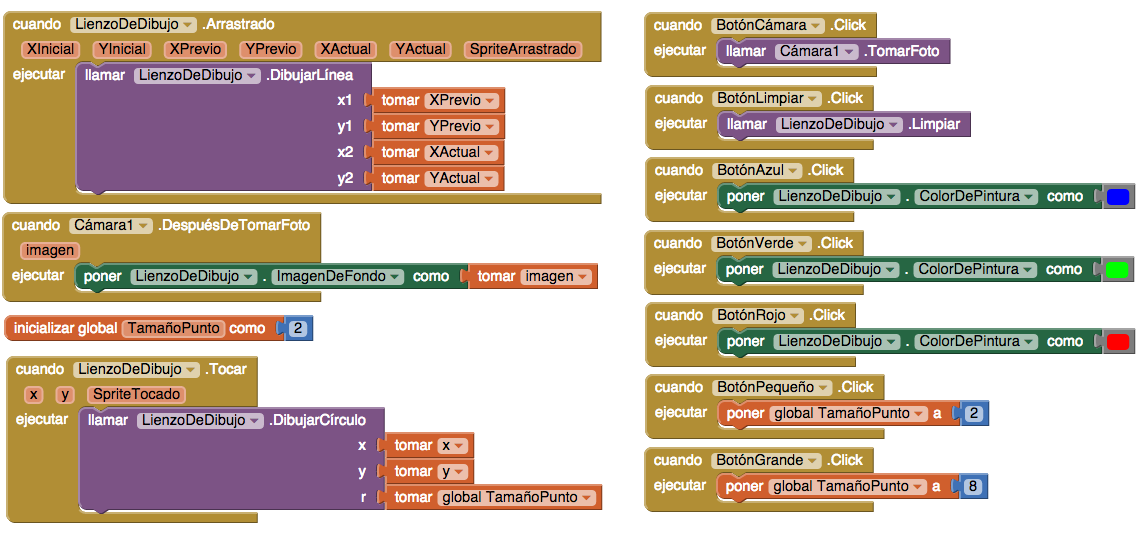
\includegraphics[scale=0.4]{PaintPot18}
\caption{Grupos de bloques para \appName{PintaFotos}.}
\label{fig:PaintPot18}
\end{figure}


\subsubsection*{Resumen}

Las ideas claves que hemos visto en este tutorial son las siguientes:

\begin{itemize}

\item El componente \component{Lienzo} te permite dibujar en un
  lienzo. También es sensible a eventos ``touch'' y de arrastre, los
  cuales puedes aprovechar para desarrollar funcionalidades para
  dibujar.

\item Puedes usar componentes de disposición en la pantalla para
  organizar tus componentes en lugar de ponerlos todos uno debajo del
  otro.

\item Algunos controladores de eventos vienen con información sobre el
  evento, como las coordenadas de donde la pantalla fue tocada. Esta
  información está representada por argumentos. Cuando arrastras un
  controlador de eventos que tiene argumentos, \AppInventor crea ítems
  ``poner a'' y ``tomar'', dentro del bloque seleccionado, para así
  poder referirse a estos argumentos.

\item Crear variables al usar bloques \block{poner global nombre},
  desde la categoría ``Variables''. Las variables permiten guardar
  información en memoria, como el tamaño del punto, que no está
  guardado en una propiedad de un componente.

\item Para cada variable que definas, \AppInventor automáticamente
  provee una referencia ``tomar global'' que entrega el valor de la
  variable, y una referencia ``poner global a'' para cambiar el valor
  de la variable. Para acceder a esto, arrastra un bloque ``poner a''
  o ``tomar'' desde el mismo bloque donde declaras la variable.
\end{itemize}

El componente Lienzo también se puede usar para programar animaciones
como las que ves en juegos en 2D.

\section{Discusión y Ejercicios de Personalización}

\paragraph{Preguntas/Discusión}

\begin{enumerate}

\item En el \component{Lienzo}, los controladores de eventos \block{Tocar} y
\block{Arrastrado}, mostrados abajo en la~\Cref{fig:PaintPot19},
tienen parámetros de evento. Nombra cada parámetro e indica lo que
representa.

\begin{figure}[H]
\centering
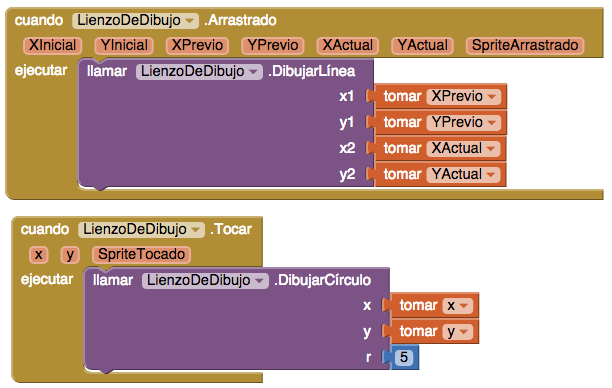
\includegraphics[scale=0.5]{PaintPot19}
\caption{Grupos de bloques para \appName{PintaFotos}.}
\label{fig:PaintPot19}
\end{figure}

\item Los parámetros de evento son distintos de los parámetros para llamar
funciones. ¿Cómo se llaman los parámetros para llamar funciones en el
controlador de eventos de la~\Cref{fig:PaintPot20}? ¿Quién especifica
los parámetros de función? Quién especifica parámetros de eventos?

\item ¿Cuál es el propósito de definir una variable para el Tamaño de Punto
en la App Pinta Fotos? Si quieres permitir cambiar el grosor de las
líneas, ¿necesitarás una variable?

\item Define lo que es una variable. ¿Cuáles son sus puntos en común con una
propiedad? ¿Cómo se diferencia de una propiedad?

\item Una forma de personalizar la aplicación es poner un
  \component{CuadroDeTexto} para el tamaño del punto. ¿Cuál es la
  diferencia entre un cuadro de texto y una variable? ¿Cuál es la
  diferencia entre una etiqueta y un cuadro de texto?

\end{enumerate}

\paragraph{Ejercicios de Personalización}

\begin{enumerate}

\item La interfaz de usuario de \appName{PintaFoto} no permite mostrar
  con qué color se está dibujando. El usuario sólo se da cuenta al
  dibujar. ¿Puedes agregar esta información para el usuario de tal
  manera que cuando él hace click para cambiar el color, la interfaz
  cambia y le indica qué color fue elegido?

\item El tamaño del punto para dibujar un círculo sólo puede ser de 2
  o 8.  ¿Puedes cambiar esto para permitir al usuario elegir entre
  distintas opciones con un componente \component{Deslizador} o un
  \component{CampoDeTexto}?

\item Permitir al usuario controlar el grosor de las líneas, de la
  misma manera que puede cambiar el tamaño del punto. El lienzo tiene
  una propiedad \property{AnchoDeLinea} que controla esta
  característica.
\end{enumerate}

\section{Tutorial: Atrapa el Topo}

En este tutorial desarrollarás el juego \emph{Atrapa el Topo},
inspirado en las salas de juegos clásicas, en las que unos topos
mecánicos saltan fuera de su hueco, y los jugadores ganan puntos
golpeándolos con un mazo. El juego fue creado por Ellen Spertus, un
miembro del equipo de \AppInventor en Google, para implementar la
funcionalidad \emph{Sprite}. El término Sprite apareció en la
comunidad de informáticos en los años 70, y se refería a imágenes
capaces de moverse en la pantalla de un computador (para videojuegos).

\subsection*{Qué Construirás}

Para la aplicación \appName{Atrapa el Topo}, ilustrada en
la~\Cref{fig:MoleMash1}, implementarás las siguientes funcionalidades:

\begin{itemize}

\item Un topo que salta en cualquier lugar de la pantalla, moviéndose
  cada segundo.

\item Tocar el topo hace vibrar el teléfono, y aumenta el marcador de
  puntos (un punto por topo tocado), y el topo se mueve de inmediato a
  otro lugar.

\item Tocar la pantalla sin alcanzar a tocar el topo provoca que el
  marcador de toques perdidos aumente.

\item Al presionar el botón ``Reiniciar'' se reinicia el contador de
  golpes logrados y perdidos.

\end{itemize}

\begin{figure}[H]
\centering
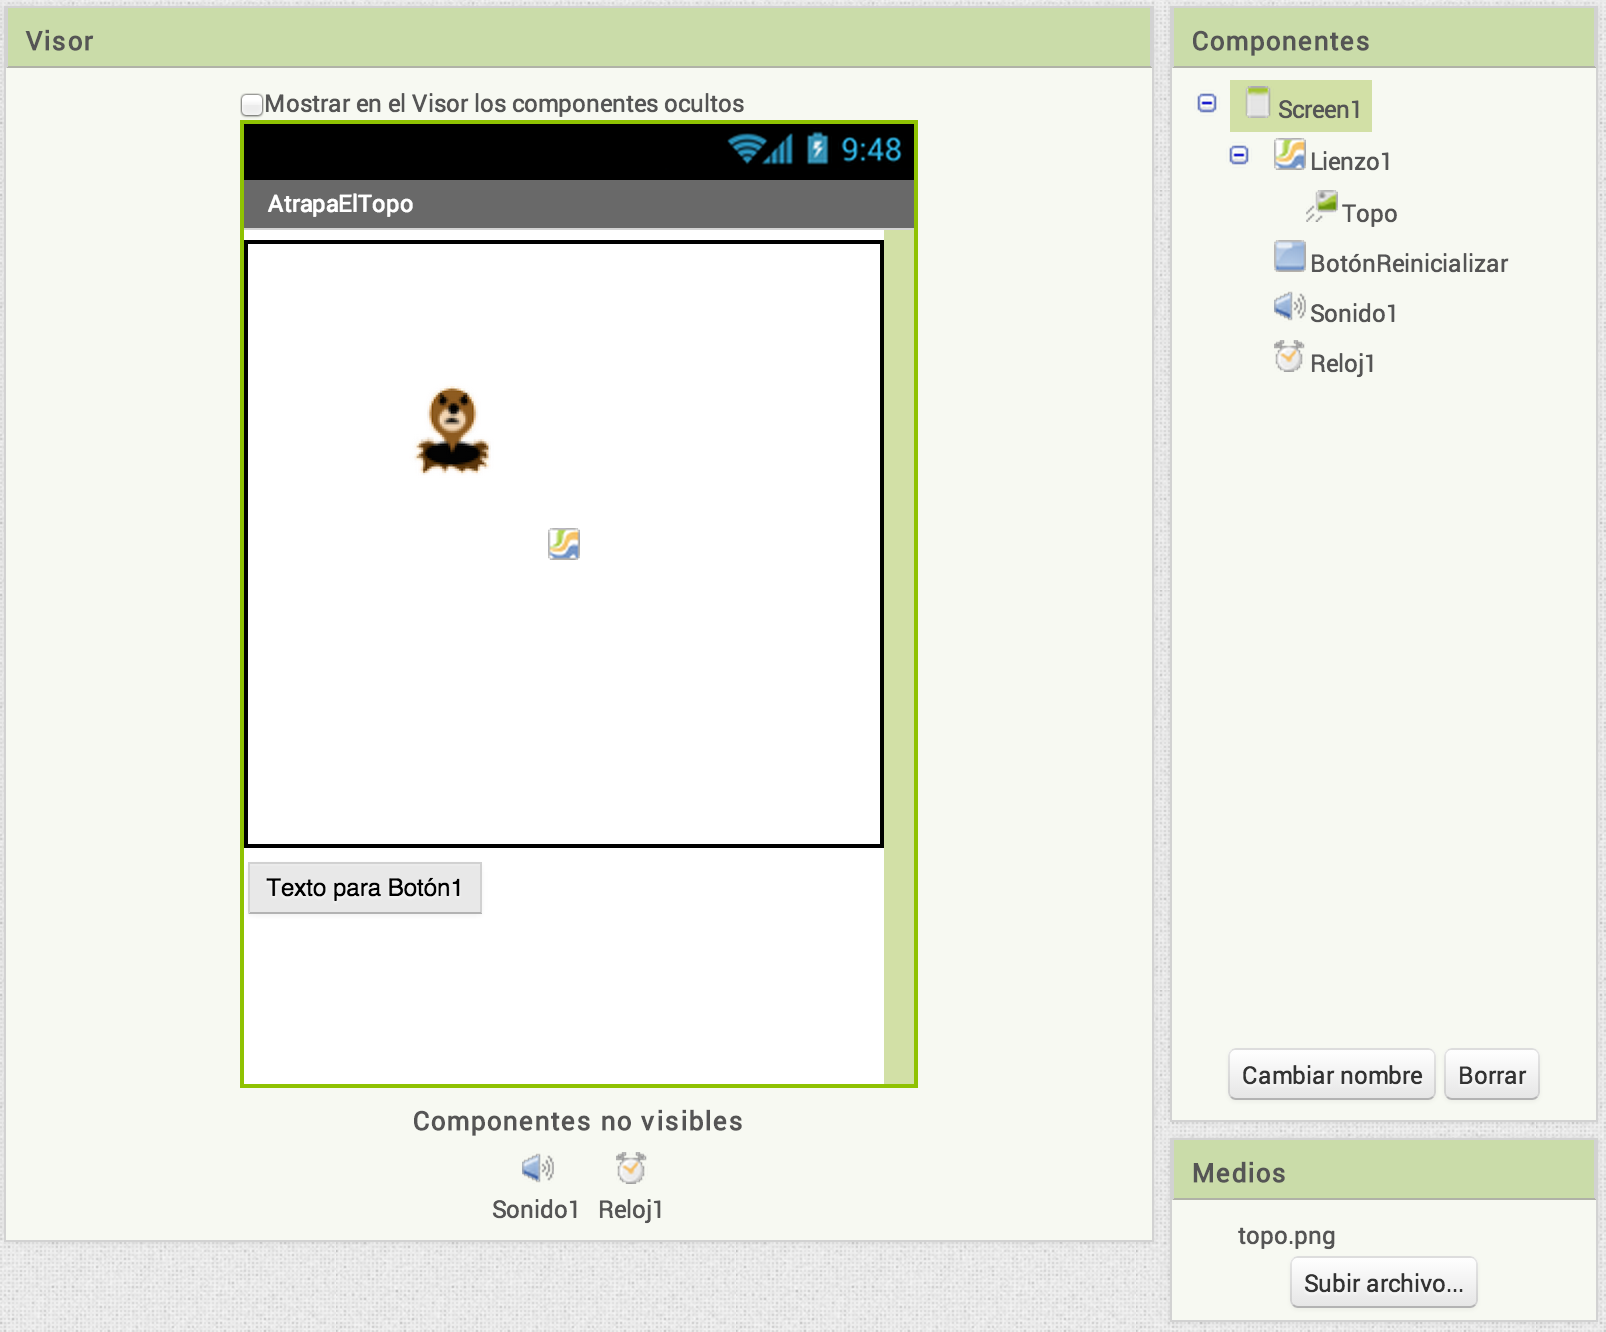
\includegraphics[scale=0.5]{MoleMash1}
\caption{ Interfaz de usuario de \appName{Atrapa el Topo}.}
\label{fig:MoleMash1}
\end{figure}


\subsection*{Qué Aprenderás}

Este tutorial cubre los siguientes componentes y conceptos:

\begin{itemize}

\item El componente \component{SpriteImagen} para imágenes movibles
  con sensibilidad touch.

\item El componente \component{Lienzo} que funciona como una
  superficie sobre la cual se pone el \component{SpriteImagen}.

\item El componente \component{Reloj} para mover el sprite.

\item El componente \component{Sonido} para producir una vibración
  cuando el topo es tocado.

\item El componente \component{Botón} para empezar un nuevo juego.

\item \emph{Procedimientos} para implementar comportamientos
  repetitivos, como desplazar el topo.

\item Generar números al azar.

\item Usar los bloques de sumar (+) y restar (-).
\end{itemize}

\subsection*{Para empezar}

Conéctate al sitio de \AppInventor y crea un nuevo proyecto. Llamálo
``AtrapaElTopo'' y también cambia el título de la pantalla como
``AtrapaElTopo''. Abre el \blockEditor y conéctate a tu dispositivo Android.

Descarga la imagen \resources{ProgramaTusIdeas/Dia2/topo.png}. Luego vé
a la sección de \media del \componentDesigner y súbela a \AppInventor.

\subsection*{Diseñando los Componentes}

Utilizarás los siguientes componentes para construir \appName{Atrapa
  el Topo}:

\begin{itemize}

\item Un \component{Lienzo} que sirve de campo de juego.

\item Un \component{SpriteImagen} que representa la foto del topo y
  que puede moverse y sentir cuando el topo fue tocado.

\item Un \component{Sonido} que vibra cuando el topo es tocado.

  \item \component{Etiquetas} que dicen ``Logrado'', ``Perdido'', y el
    número de toques logrados y pérdidos.

  \item Un componente \component{DisposiciónHorizontal} para
    posicionar las etiquetas correctamente.

  \item Un \component{Botón} para reiniciar a 0 el número de golpes
    exitosos y fallidos.

  \item Un \component{Reloj} para hacer que el topo se desplace una
    vez por segundo.
\end{itemize}

La~\Cref{tab:MoleMashTab1} muestra la lista completa de componentes
para \appName{Atrapa el Topo}.

\begin{footnotesize}
  \begin{table}[H]
    \centering
    \begin{tabular}{|p{3cm}|c|c|p{3.5cm}|}
      \hline
      % \textbf{Tipo de  Componente} & \textbf{Sección en la \palette} & \textbf{Nombre} & \textbf{Propósito}\\
      % \hline
      % Botón & Interfaz de usuario & Botón1 & Presionar para que el gato maulle.\\
      % \hline
      % Etiqueta & Interfaz de usuario & Etiqueta1 & Muestra el texto ``Hola Gatito''.\\
      % \hline
      % Sonido & Medios & Sonido1 & Reproduce el sonido del maullido.\\
      \hline
    \end{tabular}
    \caption{Lista completa de componentes para \appName{Atrapa el Topo}}
    \label{tab:MoleMashTab1}
  \end{table}
\end{footnotesize}

\subsubsection*{Ubicar los Componentes de Acción}

En esta sección crearemos los componentes necesarios para que funcione
el juego. En la siguiente sección, crearemos los componentes para
mostrar el marcador de puntos.

\begin{enumerate}

\item Arrastra un componente \component{Lienzo}, dejando su nombre por
  defecto \component{Lienzo1}. Configura sus propiedades de
  \property{Ancho} como ``Ajustar al contenedor'' y ajusta su
  \property{Alto} a 300 pixeles.

\item Arrastra un componente \component{SpriteImagen} desde el grupo
  ``Animaciones'' de la \palette. Ponlo en cualquier lugar del
  \component{Lienzo1}, y luego cambia su nombre a ``Topo''. Configura
  su propiedad de \property{Imagen} usando la imagen
  \mediafile{topo.png} que subiste anteriormente.

\item Arrastra un \component{Botón} debajo de Lienzo1. Cambia su
  nombre por ``BotónReinicializar'' y configura su \property{Texto}
  como ``Reinicializar''.

\item Arrastra un componente \component{Reloj}. Aparecerá abajo del
  \viewer, en la sección de componentes no visibles.

\item Arrastra un componente \component{Sonido}. También aparecerá
  abajo del \viewer, en la sección de componentes no-visibles.
\end{enumerate}

Tu pantalla debería verse como en la~\Cref{fig:MoleMash2} (aunque tu
topo puede estar en una posición distinta).

\begin{figure}[H]
\vspace{3em}
\centering
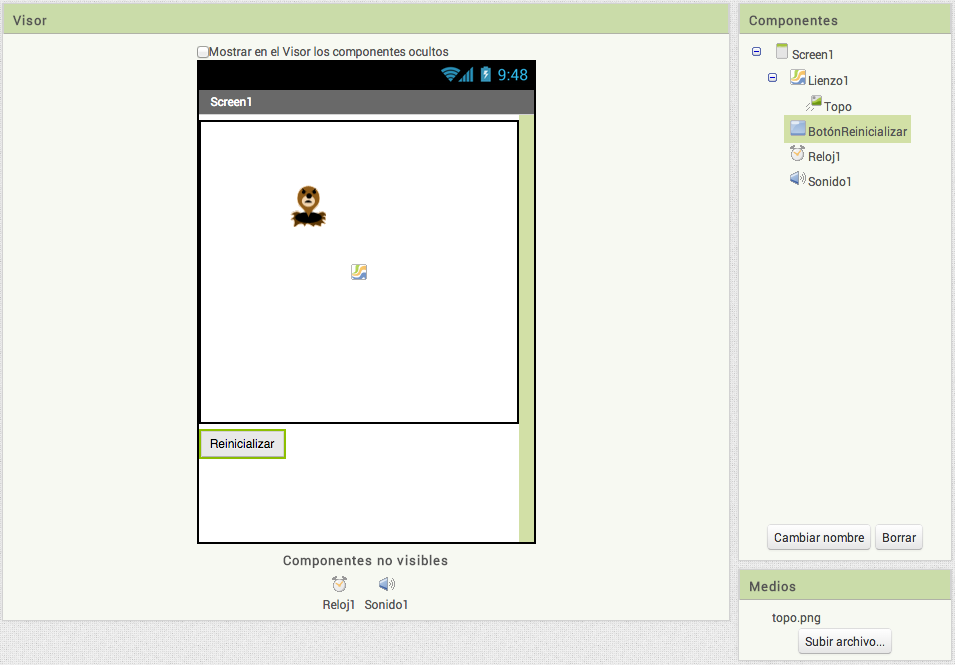
\includegraphics[scale=0.5]{MoleMash2}
\caption{El \designer con la vista de los componentes de acción}
\label{fig:MoleMash2}
\end{figure}


\subsubsection*{Poner las Etiquetas}

Ahora pondremos los componentes para mostrar el marcador de puntos del
usuario, más específicamente los golpes exitosos y fallidos.

\begin{enumerate}

\item Arrastra un componente \component{DisposiciónHorizontal}, del
  grupo ``Disposición'', poniéndolo debajo del
  \component{BotónReinicializar} y dejando el nombre por defecto
  ``DisposiciónHorizontal1''.

\item Arrastra dos \component{Etiquetas} hacia la
  \component{DisposiciónHorizontal}.

  \begin{itemize}
  \item Cambia el nombre de la etiqueta izquierda por
    ``EtiquetaExitos'' y configura su \property{Texto} como ``exitos:
    '' (\emph{Ojo!}: tienes que incluir un espacio después de los dos
    puntos).

\item Cambia el nombre de la etiqueta derecha por
  ``EtiquetaPuntosGanados'' y configura su \property{Texto} como
  ``0''.
  \end{itemize}

\item Arrastra un segundo componente
  \component{DisposiciónHorizontal}, poniendolo debajo de
  \component{DisposiciónHorizontal1}.

\item Arrastra dos \component{Etiquetas} hacia la
  \component{DisposiciónHorizontal2}
\end{enumerate}

\begin{itemize}
\item Cambia el nombre de la etiqueta izquierda por ``EtiquetaFallos''
  y configura su \property{Texto} como ``Fallos: '' (\emph{Ojo!}:
  tienes que incluir un espacio después de los dos puntos).

\item Cambia el nombre de la etiqueta derecha por
  ``EtiquetaPuntosFallados'' y configura su propiedad de
  \property{Texto} como ``0''.
\end{itemize}

Tu pantalla debería ser parecida a la~\Cref{fig:MoleMash3}

\begin{figure}[H]
\centering
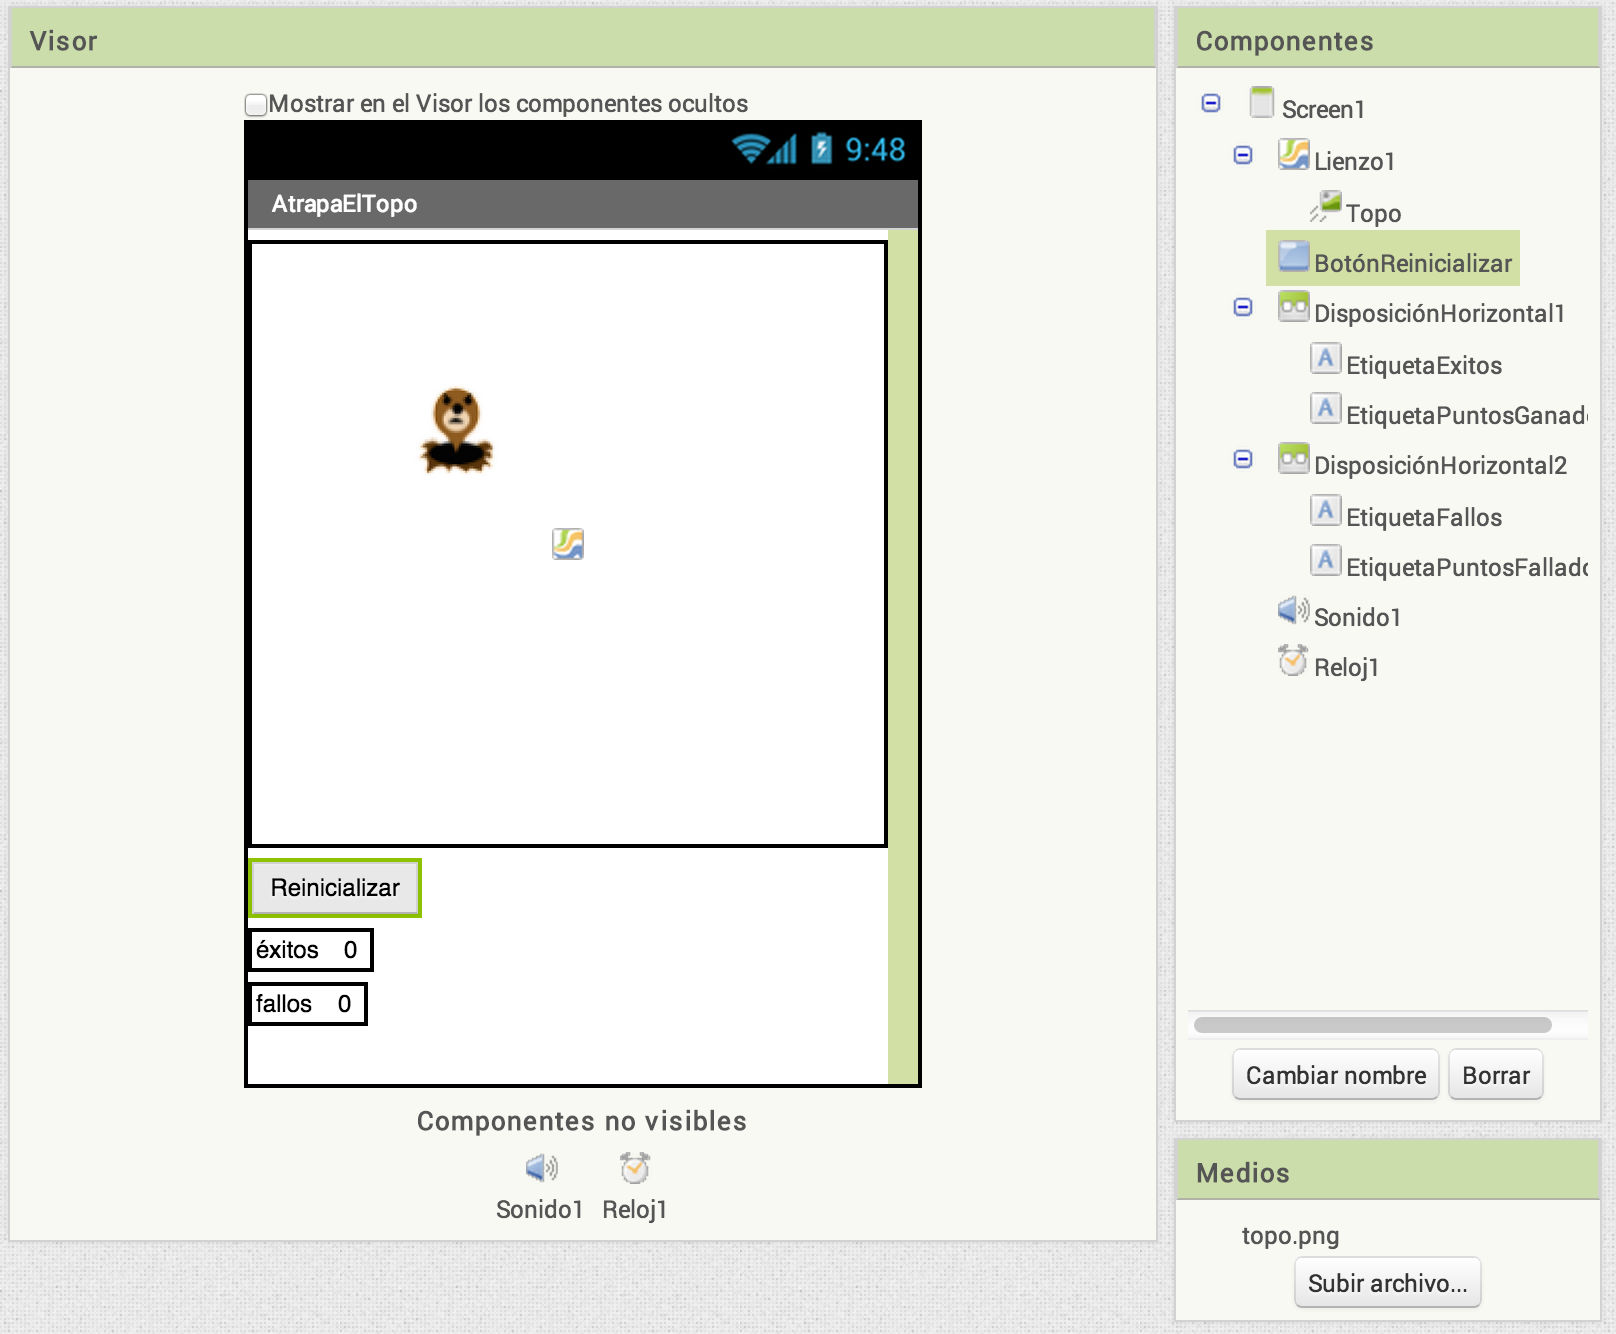
\includegraphics[scale=0.5]{MoleMash3}
\caption{El \designer con todos los componentes del juego.}
\label{fig:MoleMash3}
\end{figure}

\subsubsection*{Agregar comportamientos a los componentes}

Luego de crear los componentes anteriores, tienes que ir al
\blockEditor para implementar el comportamiento del programa. En
particular, queremos que el topo se mueva cada segundo de manera
aleatoria en el lienzo. El objetivo del jugador es pegar al topo donde
aparezca, y la aplicación mostrará el número de veces que el jugador
logró tocar o no al topo. Pinchar en el botón ``Reinicializar'',
reinicializa el marcador.

\subsubsection*{Desplazar el Topo}

En los programas que creaste hasta ahora, usaste procedimientos
preexistentes como el vibrador en \appName{Hola Gatito}. Sería
maravilloso poder tener un procedimiento que mueve un
\component{SpriteImagen} de forma aleatoria en la pantalla! La mala
noticia es que no existe! La buena noticia: puedes crear tus propios
procedimientos! Como los preexistentes, tu procedimiento aparecerá en
una sección y podrá ser usado en cualquier lugar de la app.

En particular, crearemos un procedimiento para mover el topo a un
lugar aleatorio en la pantalla, que llamaremos
\procedure{MoverTopo}. Vamos a activar \procedure{MoverTopo} al inicio
del juego, cuando el usuario logra tocar el topo, y una vez por
segundo.

\subsubsection*{Crear el procedimiento \procedure{MoverTopo}}

Para comprender cómo mover el topo, necesitamos ver cómo funcionan los
gráficos de Android.

El lienzo (y la pantalla) son como una cuadrícula con coordenadas x
(horizontal) e y (vertical), donde las coordenadas (x,y) de la esquina
superior izquierda son (0,0). El x aumenta cuando mueves hacia la
derecha, y la y aumenta cuando vas hacia abajo, como se ilustra en
la~\Cref{fig:MoleMash4}. Las propiedades \property{X} e \property{Y}
de un \component{SpriteImagen} indican dónde debería estar su esquina
superior izquierda; es decir, el topo en la esquina superior izquierda
tiene valores de 0 para X e Y.

Para determinar los valores máximos para X e Y de tal manera que el
topo no se salga de la pantalla, necesitamos estar seguros de usar las
propiedades \property{Ancho} y \property{Alto} del \component{Topo} y
del \component{Lienzo1}. Las propiedades de \property{Ancho} y
\property{Alto} del \component{Topo} son las mismas que el tamaño de
la foto que subiste. Cuando creaste el \component{Lienzo1},
configuraste su \property{Alto} a 300 pixeles y su \property{Ancho} a
``Ajustar al Contenedor''). Si el \component{Topo} tiene un
\property{Ancho} de 36 pixeles y el \component{Lienzo} 200, la
coordenada \property{X} del lado izquierdo del topo puede ir hasta 0
(borde izquierdo) o con un alto de hasta 164 (200 - 36, o
$\block{Lienzo1.Ancho} - \block{Topo.Ancho}$) sin que el topo
pase el borde derecho de la pantalla.

De forma similar, la coordenada \property{Y} del lado superior del
topo puede ir desde 0 hasta $\block{Lienzo1.Alto} -
\block{Topo.Alto}$.

\begin{figure}[H]
\centering
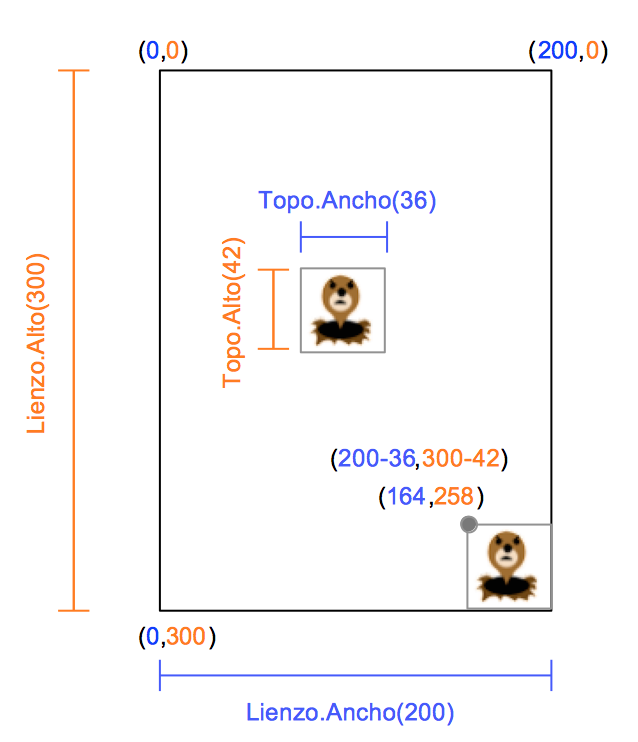
\includegraphics[scale=0.5]{MoleMash4}
\caption{Posiciones del topo en la pantalla, con información de ancho,
  coordenadas y altura. La información de la coordenada x está en
  azul, y la de la coordenada y está en naranjo.}
\label{fig:MoleMash4}
\end{figure}

Para dar una posición aleatoria al topo, vamos a seleccionar una
coordenada \property{X} entre 0 y $\block{Lienzo1.Ancho} -
\block{Topo.Ancho}$. Asímismo, la
coordenada \property{Y} tiene que estar en un rango de entre 0 y
$\block{Lienzo1.Alto} - \block{Topo.Alto}$. {Podemos generar un número aleatorio con el procedimiento
preexistente \block{entero aleatorio entre}, que se encuentra en la
sección ``Matemáticas''. Tendrás que cambiar los parámetros como se
muestra en la~\Cref{fig:MoleMash5}. La figura muestra además
comentarios descriptivos que puedes opcionalmente agregar a tu
procedimiento.

\begin{figure}[H]
\vspace{3em}
\centering
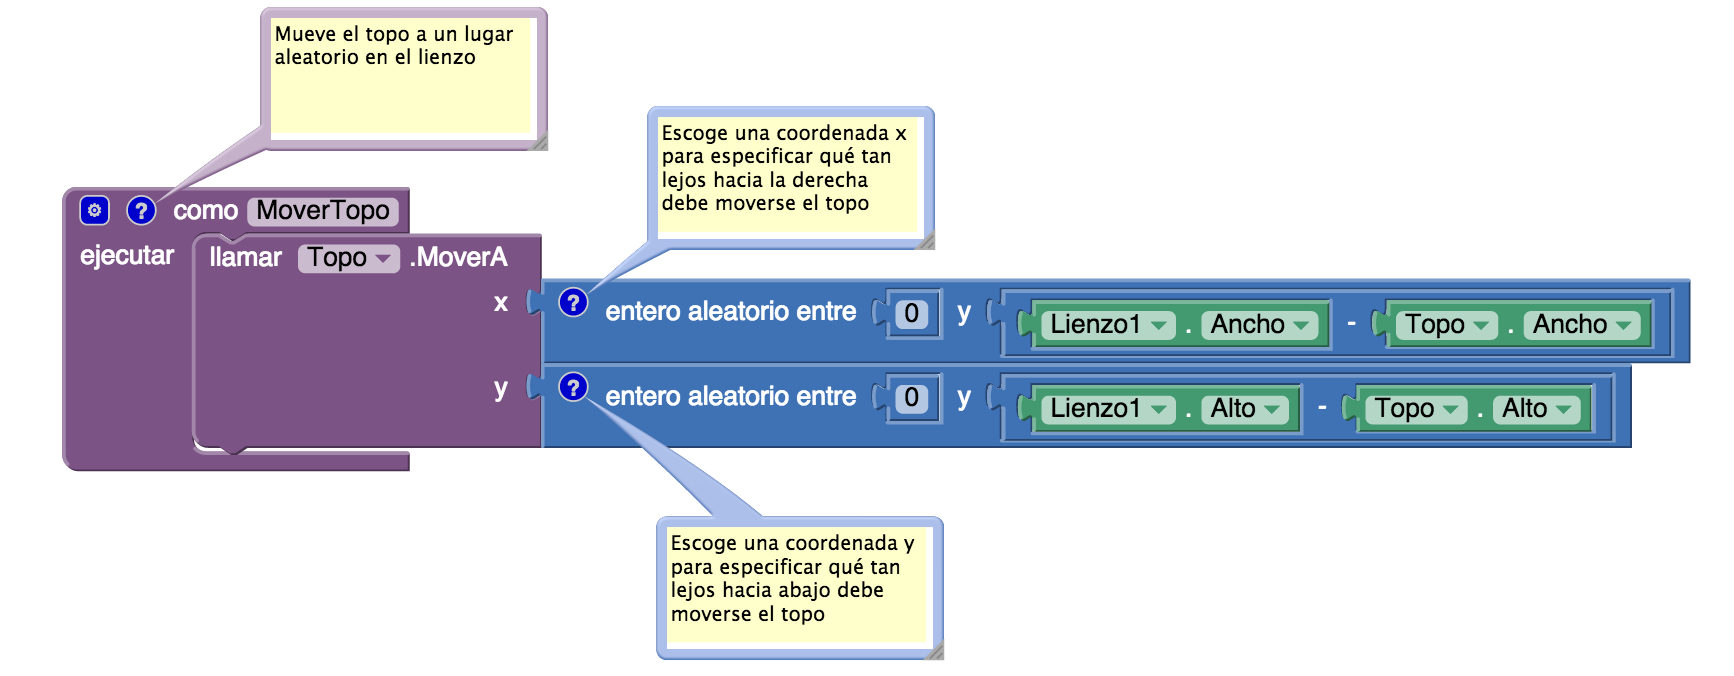
\includegraphics[scale=0.5]{MoleMash5}
\caption{El procedimiento \procedure{MoverTopo}, que pone el Topo en
  una ubicación aleatoria.}
\label{fig:MoleMash5}
\end{figure}

Para crear el procedimiento \procedure{MoverTopo}:

\begin{enumerate}

\item Selecciona la sección ``Procedimientos'' del \blockEditor.

\item Arrastrar el bloque \block{como procedimiento} (no el
  \block{como procedimiento resultado}) al espacio de trabajo.

\item Presiona el texto ``procedimiento'' en este nuevo bloque y
  reemplázalo por ``MoverTopo'', para configurar el nombre del nuevo
  procedimiento.

\item Dado que queremos mover el topo, arrastra dentro del
  procedimiento el bloque \block{llamar Topo.MoverA}, a la derecha de
  ``ejecutar''. Observa que se requiere indicar las
  coordenadas \parameter{x} e \parameter{y} donde se moverá el topo.

\item Para especificar que la nueva coordenada \parameter{x} para el topo debería ser
  entre 0 y $\block{Lienzo1.Ancho} -  \block{Topo.Ancho}$, debes hacer lo siguiente:

\begin{itemize}

\item Seleccionar la sección ``Matemáticas''.
\item Arrastra el bloque \block{entero aleatorio entre}, conectándolo
  con el parámetro \parameter{x} en \block{llamar Topo.MoverA}.
\item Cambia el número 1 en el espacio ``entre'' por un 0.
\item Borra el número 100 en el espacio ``y''.
\item Selecciona la sección ``Matemáticas'' y arrastra un bloque de
  resta (-) al espacio de trabajo.
\item Selecciona el bloque \block{Lienzo1.Ancho} y arrástralo al
  argumento izquierdo del bloque de resta.
\item De manera muy similar, arrastra el bloque \block{Topo.Ancho}
  hacia el argumento derecho del bloque de resta.
\end{itemize}

Sigue un procedimiento similar para especificar que la coordenada
y, que debería ser un entero aleatorio entre 0 y
$\block{Lienzo1.Alto} - \block{Topo.Alto}$.

\end{enumerate}

Compara tus resultados con lo ilustrado en la~\Cref{fig:MoleMash5} que
está más arriba.

\subsubsection*{Llamar \procedure{MoverTopo} cuando se Inicia la Aplicación}

Ahora que escribiste el procedimiento \procedure{MoverTopo}, ¡usémoslo!
Es muy común que los programadores quieran que pase algo cuando se
inicia la aplicación, y es por eso que hay un bloque para esto: \block{Pantalla1.Inicializar}.

\begin{enumerate}

\item Arrastra el bloque \block{Pantalla1.Inicializar}, desde la
  sección \component{Pantalla1}.

\item Selecciona la sección ``Procedimientos'', donde ahora verás un
  bloque llamado \block{llamar MoverTopo} (¿Te das cuenta que tú
  creaste este bloque?!). Arrastra el bloque y ponlo dentro de
  \block{Pantalla1.Inicializar}, como se muestra en
  la~\Cref{fig:MoleMash6}.

\begin{figure}[H]
\centering
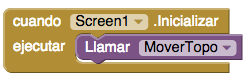
\includegraphics[scale=0.5]{MoleMash6}
\caption{Llamar el procedimiento MoverTopo cuando se inicia la
aplicación.}
\label{fig:MoleMash6}
\end{figure}

\end{enumerate}


\subsubsection*{Llamar a \procedure{MoverTopo} cada 1 Segundo}

Hacer que el topo se mueva cada 1 segundo requiere que usemos el
componente \component{Reloj}. Dejamos la propiedad
\property{IntervaloDelTemporizador} en su valor por defecto de 1000
milisegundos (o sea 1 segundo). Esto significa que cada 1 segundo se
ejecutará un evento \block{Reloj1.Temporizador}. Estos eventos los
usaremos para mover el topo cada 1 segundo, de la siguiente manera:

\begin{enumerate}

\item Selecciona la sección \component{Reloj1}, y arrastra el
  controlador de eventos \block{Reloj1.Temporizador} hacia el espacio
  de trabajo.

\item Arrastra un bloque \block{llamar MoverTopo}, desde la sección
  ``Procedimientos'', hacia el interior del controlador de eventos
  \block{Reloj1.Temporizador}, como se muestra en
  la~\Cref{fig:MoleMash7}.

\begin{figure}[H]
\centering
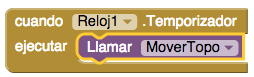
\includegraphics[scale=0.5]{MoleMash7}
\caption{Procedimiento para llamar a \procedure{MoverTopo} cada 1
  segundo, cada vez que se activa el temporizador.}
\label{fig:MoleMash7}
\end{figure}

\end{enumerate}

Si el movimiento es demasiado lento o rápido para ti, puedes cambiar
la propiedad de intervalo de tiempo en el \designer, para cambiar la
frecuencia de movimiento.

\subsubsection*{Llevar el Puntaje}

¿Te acuerdas que creaste dos etiquetas
\component{EtiquetaPuntosGanados} y
\component{EtiquetaPuntosFallados}, con valores iniciales de 0?. Ahora
queremos incrementar los números en estas etiquetas cuando el usuario
logra tocar el topo (un éxito) o cuando toca la pantalla sin tocar el
topo (fallado). Para hacer esto, usaremos el bloque
\block{Lienzo1.Tocar}, que indica que el lienzo fue tocado, las
coordenadas x e y de donde fue tocado (lo que no es necesario saber en
este caso), y si un sprite fue tocado (lo que si necesitamos
saber). La~\Cref{fig:MoleMash8} muestra el código que vamos a crear.

\begin{figure}[H]
\centering
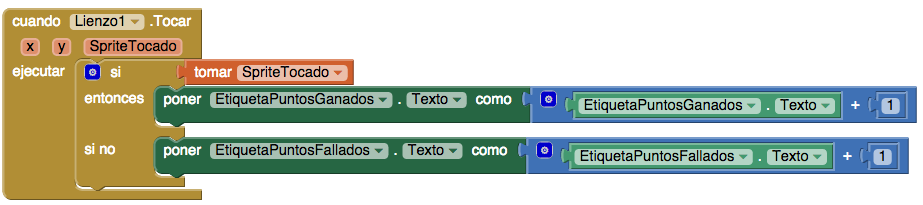
\includegraphics[scale=0.5]{MoleMash8}
\caption{Se incrementa el número de éxitos o fallidos cuando el lienzo está tocado.}
\label{fig:MoleMash8}
\end{figure}

La traducción de la~\Cref{fig:MoleMash8} es la siguiente: cuando el
lienzo es tocado, se chequea si el sprite fue tocado. Dado que hay un
solo sprite en nuestro programa, tiene que ser \component{Topo1}. Si
el \component{Topo} es tocado, suma 1 al número en
\block{EtiquetaPuntosGanados.Texto}; sino, suma 1 al número en
  \block{EtiquetaPuntosFallados.Texto}. El valor
  de \parameter{SpriteTocado} es falso si ningun sprite fue tocado.

Los bloques se crean de la siguiente manera:

\begin{enumerate}

\item Arrastra el bloque \block{Lienzo1.Tocar}.

\item Selecciona la sección ``Control'', y arrastra un bloque
  \block{si-sino} (tendrás que agregar el bloque \block{sino} después
  de mover el bloque al espacio de trabajo) y colócalo dentro de
  \block{Lienzo1.Tocar}.

\item Arrastra un bloque \block{tomar SpriteTocado}, y ponlo en el
  espacio abierto del bloque \block{si}.

\item Dado que queremos que \block{EtiquetaPuntosGanados.Texto} sea
  incrementado si el topo fue tocado:

\begin{itemize}

\item Desde la sección \component{EtiquetaPuntosGanados}, arrastra el
  bloque \block{poner EtiquetaPuntosGanados.Texto}, y ponlo a la
  derecha de ``entonces'' en el bloque \block{si}.

\item Arrastra el bloque de suma (+), desde la sección
  ``Matemáticas'', hasta el espacio del bloque \block{poner
    EtiquetaPuntosGanados.Texto como}.

\item Arrastra el bloque \block{EtiquetaPuntosGanados.Texto} como el
  argumento izquierdo del bloque de suma.

\item Agrega un bloque numérico con valor 1 como argumento derecho del
  bloque de suma.

\end{itemize}

\item Repite el paso anterior, pero para la etiqueta
  \block{EtiquetaPuntosFallados}, en la sección \block{si no}, del
  bloque \block{si ... sino}.

  \paragraph{Prueba tu Aplicación!} Puedes probar tu juego tocando el
  lienzo y el topo, y viendo cómo cambian los puntajes.

\end{enumerate}

\subsubsection*{Abstracción procedural}

La capacidad de nombrar y luego llamar una serie de instrucciones como
\procedure{MoverTopo} es una de las herramientas claves en ciencias de
la computación, y esta herramienta se llama \emph{abstracción
  procedural}.

Se llama \emph{abstracción} porque el que llama el procedimiento
(quien, en el mundo real, por lo general es una persona distinta a la
que es el autor del procedimiento) solamente necesita saber \emph{qué}
hace el procedimiento (mover el topo), pero no \emph{cómo} lo hace (al
hacer dos llamados al generador de números aleatorios). Sin la
abstracción procedural, grandes programas de computación no serían
posibles porque contienen demasiado código para que lo memorice una
sola persona. Se puede hacer una analogía con la división del trabajo
en una planta por ejemplo, donde distintos ingenieros diseñan
diferentes partes de un auto, ninguno de ellos entendiendo todos los
detalles, y el conductor sólo tiene que comprender la interfaz (por
ejemplo apretar el freno para detener el auto), y no toda la
ingeniería que hay por detrás.

Algunas ventajas de la abstracción procedural en comparación con
copiar y pegar código son:

\begin{itemize}

\item Es más fácil probar el código si está nítidamente separado del
  resto del programa.

\item Si hay un error en el código, solamente hay que arreglarlo en un
  lugar.

\item Para cambiar el desarrollo, como por ejemplo programar que el
  topo no se mueva al lugar donde justo estuvo antes, solamente
  modificas el código en un lugar.

\item Los procedimientos pueden ser juntados en una \emph{librería} y
  usados en distintos programas (aunque no se puede hacer esto todavía
  con \AppInventor).

\item Dividir el código en trozos permite reflexionar bien sobre el
  código y desarrollar la aplicación de acuerdo a esta reflexión.

\item Elegir buenos nombres para los procedimientos ayuda a documentar
  el código, haciéndolo más fácil de leer para otra persona que lo
  tomará después.

\end{itemize}

Más adelante aprenderás a hacer procedimientos más potentes, agregando
argumentos, dando valores de retorno y haciendo que los procedimientos
se llamen a ellos mismos.

\subsubsection*{Reinicializar el Puntaje}

Si un amigo te ve jugar, ¡es probable que quiera probar el juego
también! Entonces será bueno tener una manera de reinicializar el
marcador de puntos en 0. Puede ser que logres hacer esto sin leer
estas indicaciones. Intenta hacerlo solo antes de leer las
instrucciones.

Lo que necesitamos es un bloque \block{BotónReinicializar.Click} que
ponga el marcador de \block{EtiquetaPuntosGanados.Texto} y
\block{EtiquetaPuntosFallidos.Texto} en 0. Crea los bloques de la
misma manera que en la~\Cref{fig:MoleMash9}.

\begin{figure}[H]
\centering
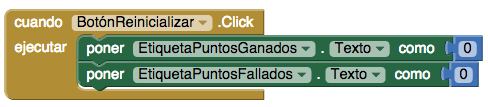
\includegraphics[scale=0.5]{MoleMash9}
\caption{Reinicializar los marcadores cuando se apreta el
botón ``Reinicializar''.}
\label{fig:MoleMash9}
\end{figure}

En esta etapa del taller, no deberías necesitar instrucciones paso a
paso para crear un controlador de eventos que responde al click de un
botón, pero aquí va un consejo para acelerar el proceso: en vez de
sacar tu número de la sección ``Matemáticas'', solamente tipea 0, y el
bloque debería crearse. (Estos atajos existen para otros bloques
también.)

\paragraph{Prueba tu Aplicación!} Intenta jugar y luego apreta el
botón ``Reinicializar''.

\subsubsection*{Agregar un Comportamiento cuando el Topo es Tocado}

Dijimos antes que queremos que vibre el dispositivo cuando se toca el
topo, lo que podemos hacer con el bloque \block{Sonido1.Vibrar}, como
se ve en la~\Cref{fig:MoleMash10}.

\begin{figure}[H]
\centering
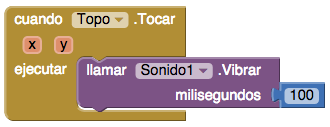
\includegraphics[scale=0.5]{MoleMash10}
\caption{Cuando el topo es tocado el dispositivo vibra brevemente
  (1000ms).}
\label{fig:MoleMash10}
\end{figure}

\paragraph{Prueba tu Aplicación!}{Revisa si vibra el teléfono cuando tocas el topo. Si
la vibración es demasiada larga o corta, según tu gusto, cambia el
número de milisegundos en el bloque \block{Sonido1.Vibrar}

\subsubsection*{La Aplicación Completa: \appName{Atrapa el Topo}}

La~\Cref{fig:MoleMash11} muestra cómo se ven los bloques para la
versión completa de \appName{Atrapa el Topo}.

\begin{figure}[H]
\vspace{3em}
\centering
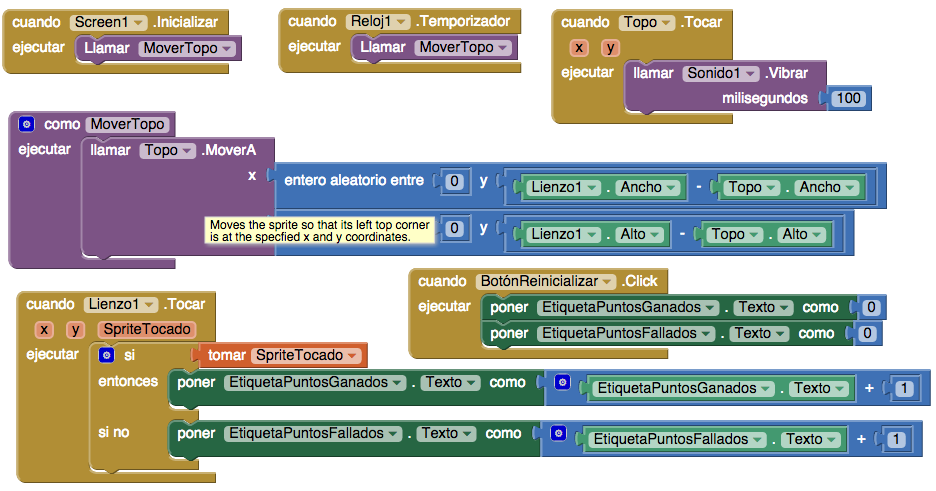
\includegraphics[scale=0.5]{MoleMash11}
\caption{El código de la versión completa de \appName{Atrapa el Topo}.}
\label{fig:MoleMash11}
\end{figure}

\subsubsection*{Variantes}

Aquí vienen algunas ideas para agregar más funcionalidades a
\appName{Atrapa el Topo}:

\begin{itemize}

\item Agregar botones para mover el topo más lento o más rápido.
\item Agregar una etiqueta para recordar y mostrar cuántas veces
  apareció el topo.
\item Agregar un segundo \component{SpriteImagen} con una foto de algo
  que el jugador \emph{NO} debería tocar, como una flor o una bomba
  por ejemplo. Si lo toca, será penalizado con puntos o puede que
  termine el juego.
\item En vez de usar la foto de un topo, deja que el usuario
  seleccione una foto con el componente
  \component{SelectorDeContacto}.
\end{itemize}

\section{Material de Apoyo}

\subsection*{El Componente Lienzo}

El componente \component{Lienzo} es una subsección dentro de tu
aplicación. El lienzo se usa para dibujar y hacer animaciones---tu app
puede dibujar objetos, y puedes dar al usuario la capacidad de dibujar
objetos.

Normalmente vas a necesitar que el lienzo llene por completo el ancho
de la pantalla de la app, entonces tendrás que ajustar la propiedad
\property{Ancho} con la opción ``Ajustar al contenedor''. Por lo
general vas a necesitar tener otros elementos abajo o arriba, por lo
que configurarás el \property{Alto} como un número fijo de pixeles.

La ubicación de un objeto en el lienzo se define con coordenadas
\property{X}, \property{Y} relativas a la esquina arriba e izquierda
del lienzo. \property{X} es la ubicación horizontal del objeto, siendo
0 el borde izquierdo y \property{X} creciendo cuando el objeto se
mueve hacia la derecha. \property{Y} es la ubicación vertical, con 0
siendo el borde superior e \property{Y} creciendo cuando el objeto se
mueve hacia abajo. Conceptualmente el lienzo se comporta como una
rejilla, tal como se ilustra en la~\Cref{fig:Lienzo}.

\begin{figure}[H]
\centering
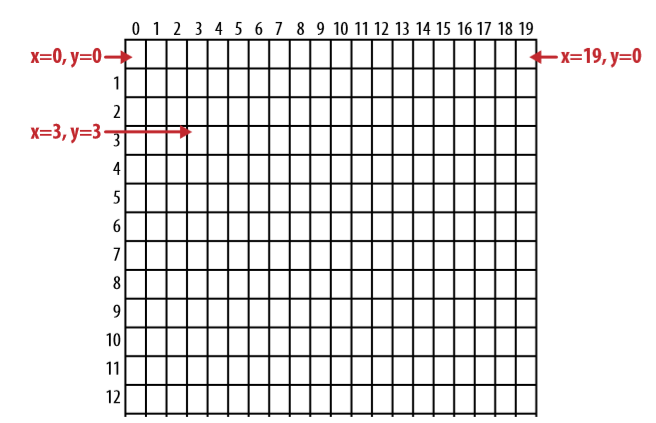
\includegraphics[scale=0.5]{Lienzo}
\caption{Un lienzo con ancho de 19 pixeles y altura de 12 pixeles. Se
  muestran los puntos en coordenadas (0,0), (3,3) y (19, 0).}
\label{fig:Lienzo}
\end{figure}

\paragraph{Ejemplo: ¿Cómo dibujar un círculo en (10,10)?}

El lienzo tiene bloques funcionales para dibujar un círculo o una
línea. El círculo tiene tres parámetros \parameter{x}, \parameter{y} y
un radio \parameter{r}. \parameter{x} es la ubicación
horizontal, \parameter{y} es la ubicación vertical, y \parameter{r} es
el radio del círculo por dibujar. Si \parameter{x} tiene un valor de
10 significa que el círculo será ubicado {10 pixeles a la derecha del
  borde izquierdo del lienzo. Si \parameter{y} tiene un valor de 10
  significa que el círculo será ubicado 10 pixeles abajo del borde
  superior del lienzo. La~\Cref{fig:DrawCircle} muestra cómo dibujar
  un círculo en la coordenada (10,10) y con radio de 5 pixeles.

\begin{figure}[H]
\centering
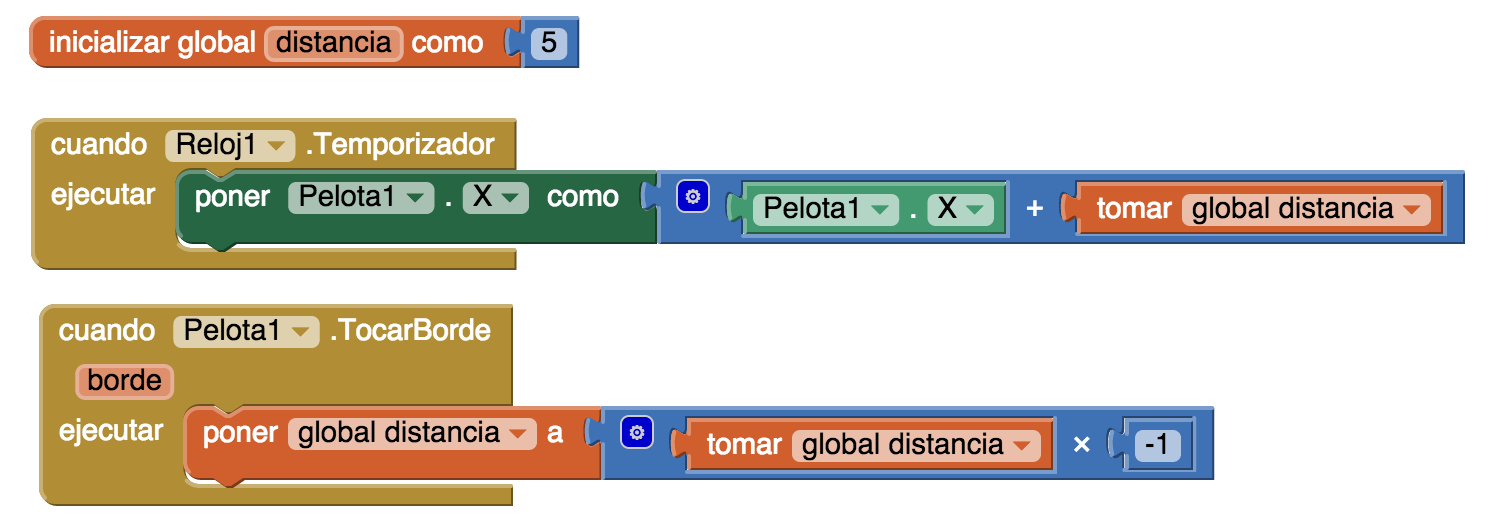
\includegraphics[scale=0.5]{DrawCircle}
\caption{Dibujando un círculo en el lienzo, en la coordenada (10,10) y
  con radio 5 pixeles.}
\label{fig:DrawCircle}
\end{figure}

\paragraph{Ejemplo: ¿Cómo dibujar un círculo en el lugar donde el
  usuario toca el lienzo?}

La funcionalidad ``touch'' (táctil) se activa cuando el usuario toca
con el dedo en el lienzo. Tiene parámetros \parameter{x}
e \parameter{y} que indican la ubicación del toque. El
parámetro \parameter{SpriteTocado} especifica si el toque ocurrió o no
en un \component{SpriteImagen} (esto no influye en su comportamiento).

Para dibujar el círculo donde el usuario tocó el lienzo, debes pasar
el mouse sobre los parámetros \parameter{x} e \parameter{y} para
arrastrar los bloques \block{tomar} para cada uno, y luego conectarlos
en los espacios para \parameter{x} e \parameter{y} del bloque
\block{DibujarCírculo}. No te confundas con lo siguiente: los
parámetros del evento \block{Tocar}} tienen el mismo nombre que los espacios
libres para especificar la ubicación del círculo en
\block{DibujarCírculo}, pero son valores independientes y con
conceptualización diferente. La~\Cref{fig:TouchDrawCircle} muestra el
código descrito anteriormente.

\begin{figure}[H]
\centering
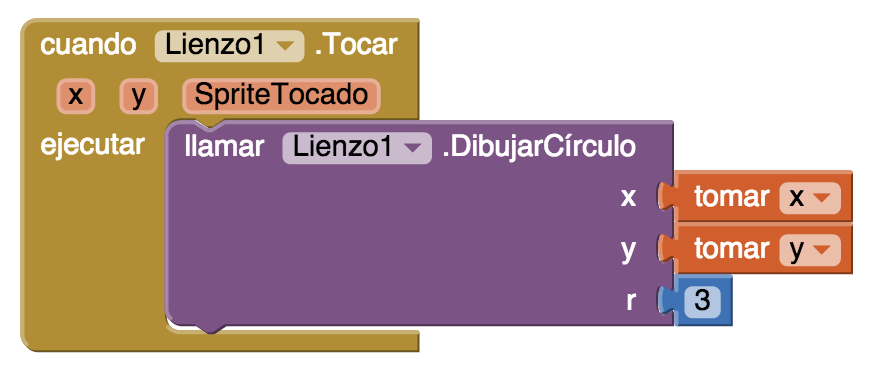
\includegraphics[scale=0.5]{TouchDrawCircle}
\caption{Dibujando un círculo en el lugar donde el usuario toca el lienzo.}
\label{fig:TouchDrawCircle}
\end{figure}

\paragraph{Ejemplo: ¿Cómo mover una imagen al centro del lienzo?}

Los bloques de la~\Cref{fig:CenterSprite} ubican el
\component{SpriteImagen1} en el centro del lienzo usando las
propiedades \property{Ancho} y \property{Alto}. Dichas referencias
abstractas significan que el código funcionará aunque el lienzo cambie
de tamaño.

\begin{figure}[H]
\centering
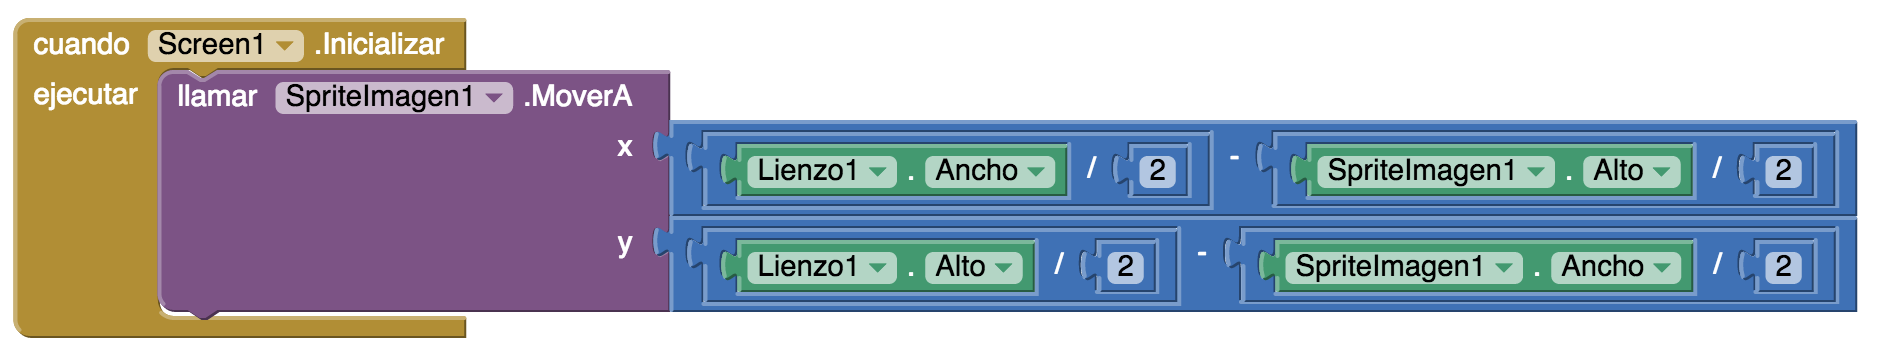
\includegraphics[scale=0.5]{CenterSprite}
\caption{Código para posicionar un sprite en el centro del lienzo.}
\label{fig:CenterSprite}
\end{figure}

Una alternativa es poner números fijos para \property{X} e
\property{Y}, después del bloque \block{SpriteImagen1.MoverA}. Es muy
similar a como (10, 10) fue usado en el ejemplo anterior. ¿Sabes
porqué es sustraída la mitad del alto y ancho del sprite?

Fijáte que no existe un bloque \block{DibujaImagen} como
\block{DibujarCírculo}. En vez de eso, con el \designer arrastras los
componentes \component{SpriteImagen} en un lienzo y especificas la
imagen (una foto) que define su apariencia.  No hay forma de crear
sprites dinámicos con bloques, sólo se pueden hacer visibles o
invisibles, y se puede cambiar su ubicación, tal como se muestra en
este ejemplo.

\subsection*{Variables}

\paragraph{¿Cuándo defines una variable?}

Una aplicación memoriza cosas, tiene una memoria ``escondida''. Puedes
imaginártelo como una hoja de cálculo (o planilla) dentro del
``cerebro'' privado de la aplicación. Tú, el programador, controlas su
memoria. Cuando arrastras un componente en tu aplicación (por ejemplo
un botón, un cuadro de texto), cada componente tiene una serie de
propiedades. Estas propiedades son celdas de tu hoja de cálculo que
puedes modificar.

También puedes definir nuevas celdas en tu planilla, cuando necesitas
recordar algo: se llaman \emph{variables}. Defines una variable cuando
no existe en el componente una propiedad para almacenar la información
que necesitas.

\paragraph{Ejemplo: ¿Cómo hacer para que cada vez que el usuario hace click se agranda el círculo?}

Como se ilustra en la~\Cref{fig:Variables1}, cuando se toca el
\component{Lienzo1} se llama a \block{Lienzo1.DibujarCírculo} para
dibujar un círculo donde se hizo el touch, en las coordenadas (x,
y). El radio \parameter{r} no puede ser un número fijo si queremos un
tamaño de círculo distinto cada vez. La variable
\variable{TamañoCírculo} se usa para seguir y recordar el tamaño de
los círculos cada vez que se dibuja uno. Se inicializa
\variable{TamañoCírculo} en 1 para que el primer círculo que se dibuje
sea solo un pequeño punto. Luego, al final del controlador de eventos
\block{Lienzo1.Tocar} el tamaño del círculo se duplica. Entonces la
segunda vez el círculo tendrá un radio 2, luego 4, luego 8, etc. La
variable \variable{TamañoCírculo} se necesita porque no hay ninguna
propiedad del componente que se pueda usar. Por ejemplo, el componente
\component{Lienzo} tiene una propiedad \property{AnchoDeLínea},
entonces si estuvieses dibujando líneas no necesitarías definir una
variable porque podrías usar esta propiedad. Pero el lienzo no tiene
una propiedad ``Tamaño de Círculo'', por lo que debes definirla tú
mismo usando una variable.

\begin{figure}[H]
\centering
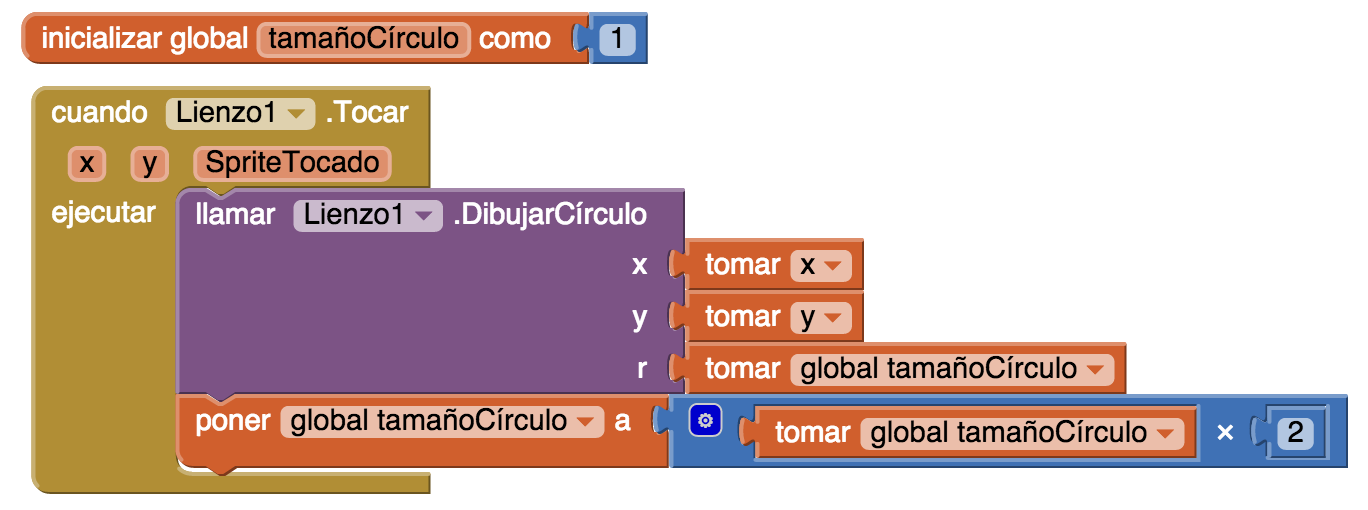
\includegraphics[scale=0.5]{Variables1}
\caption{Usando una variable para controlar el radio de los círculos dibujados.}
\label{fig:Variables1}
\end{figure}

% TODO: para día 3?
% \paragraph{Ejemplo: ¿Como hacer que una pelota cruce la pantalla?}

% {En este ejemplo, se define una variable distancia para que la app
% recuerde la dirección correcta en la cual la pelota se mueve. Quieres
% que la pelota se mueve dentro de ciertos intervalos de tiempo, entonces
% la ubicación horizontal de la pelota (Pelota1.X) se modifica y configura
% en el}{~gestionador de tiempo del Reloj1}{. La parte compleja es que no
% siempre quieres que la pelota se mueva de la misma forma. Cuando la
% pelota se mueve hacia la derecha, tienes que agregar un número positivo
% (por ej. 5) para la Pelota1.X. Cuando la pelota se mueva hacia la
% izquierda tienes que agregar un número negativo (ej. -5). El número que
% agregas a Pelota1.X es vinculado a la dirección en la cual se mueve la
% pelota.}
% {}
% {Para recordar en qué sentido se mueve la pelota, tienes que definir la
% variable distancia. Esta se inicializa en 5, entonces cuando se inicia
% la app cada ciclo}{~del contador }{permite mover la pelota hacia la
% derecha. Cuando la pelota toca el borde (derecho), se activa ``Pelota1
% Borde Alcanzado'', y la distancia se configura }{a -1 o
% -5}\textsuperscript{\hyperref[cmnt7]{{[}g{]}}\hyperref[cmnt8]{{[}h{]}}}{.
% En otras palabras, su signo se revierte.}
% {}
% {Cuando la distancia es -5, el próximo evento del contador provoca el
% desplazamiento de la pelota hacia la izquierda. Cuando la pelota toca el
% borde izquierdo, se activa nuevamente Pelota1.BordeAlcanzado, el signo
% de distancia se revierte de nuevo, a 5, y la pelota empieza nuevamente a
% moverse hacia la derecha. Este comportamiento continúa de forma que la
% pelota va y viene para siempre.~~~~~~~~}
% {~~~~~~~~~~~~~~~~}
% {Nota que hay varias maneras de programar este comportamiento de ida y
% vuelta, y se puede hacer también sin usar una variable.~~~~~~~~}
% {~~~~~~~~~~~~~~~~}


\subsection*{Temporizadores}

\subsubsection*{Actividades Temporizadas}

¿Cómo programar el tiempo? ¿Cómo programar una animación?. En otros
lenguajes de programación, los conceptos de animación se ven mucho más
adelante, pero con la metodología de \AppInventor puedes explorar este
concepto desde el inicio. El componente \component{Reloj} sirve de
alarma, y puedes usar su función de temporizador para iniciar una
actividad con tiempos específicos.

Mira los siguientes ejemplos:

\paragraph{Ejemplo: ¿Cómo tocar un sonido cada 1 segundo?}

Como muestra la~\Cref{fig:Clock1} esto se puede hacer cuando se activa
el evento \component{Reloj.Temporizador} de manera repetida. Conviene
pensar en el temporizador como una alarma, donde la propiedad
\property{Reloj.IntervaloDelTemporizador} determina cada cuanto se toca el
sonido (por defecto son 1000 milisegundos, o 1 segundo). Entonces si
no lo cambias el sonido se escuchará cada segundo. Puedes configurar
esta propiedad en el \designer o dinámicamente usando bloques.

\begin{figure}[H]
\centering
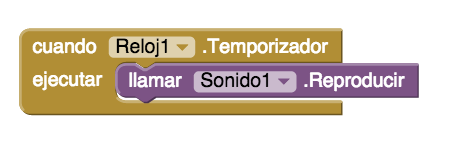
\includegraphics[scale=0.5]{Clock1}
\caption{Reproducir un sonido cada 1 segundo}
\label{fig:Clock1}
\end{figure}

\paragraph{Ejemplo 2: ¿Cómo tocar un sonido cada 5 segundos?}

Como se dijo anteriormente, la propiedad \property{Reloj.IntervaloDelTemporizador} determina cada cuanto se toca el
sonido. Por defecto esta configurado en 1000 milisegundos (1 segundo).
Si lo configuras en 5000, el evento \block{Reloj.Temporizador} se activará cada 5
segundos, como se muestra en la~\Cref{fig:Clock2}.

\begin{figure}[H]
\centering
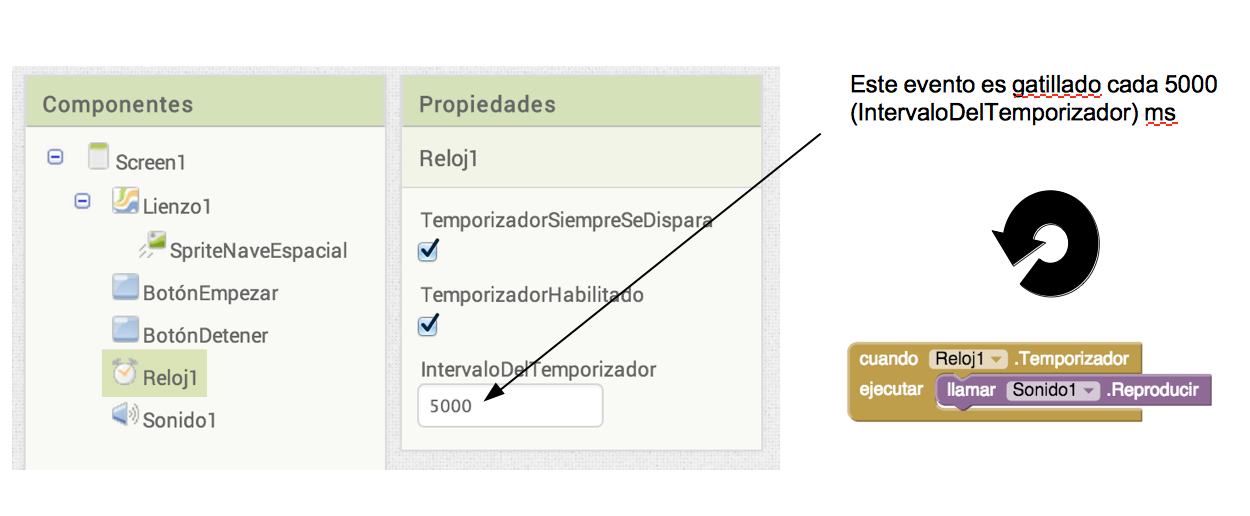
\includegraphics[scale=0.5]{Clock2}
\caption{Reproducir un sonido cada 5 segundos}
\label{fig:Clock2}
\end{figure}

Puede ser un poco confuso e indirecto tener que cambiar el intervalo
en el \designer para luego especificar el comportamiento en el
\blockEditor. La clave es comprender que el temporizador se gatillará
como un evento cada \property{Reloj.IntervaloDeTemporizador}
milisegundos.

\paragraph{Ejemplo 3: ¿Cómo desplazas una nave espacial suavemente por la pantalla?}

Asumamos que tienes un \component{SpriteImagen} que representa una
nave espacial. La coordenada \property{X} de la nave espacial define
su posición horizontal. Para generar el movimiento hay que hacer que
cada evento del temporizador aumente la coordenada \property{X}, para
que así la nave aparezca un poco más a la derecha, como se muestra en
la~\Cref{fig:Clock3}. Si el \property{IntervaloDelTemporizador} tiene
su propiedad por defecto en 1000 milisegundos, entonces la nave se
moverá cada segundo. Para este tipo de animación, configurarás el
intervalo en 40 milisegundos.

\begin{figure}[H]
\centering
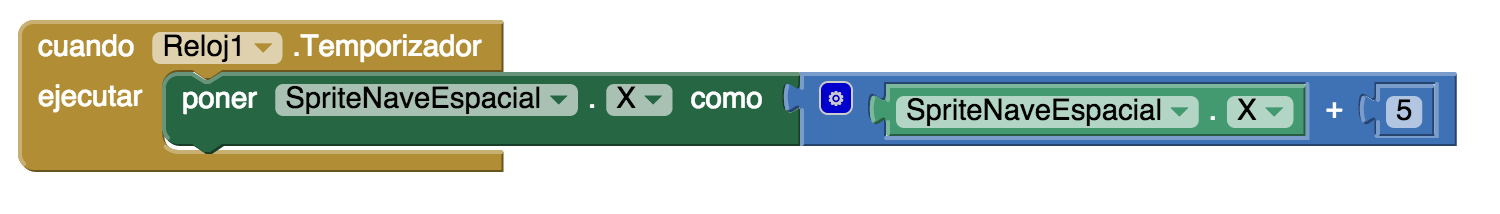
\includegraphics[scale=0.5]{Clock3}
\caption{Mover una nave espacial por la pantalla.}
\label{fig:Clock3}
\end{figure}

\paragraph{Ejemplo 4: Una película es una secuencia de imágenes que se
  muestran muy rápidamente}

La frecuencia de cuadros de una imagen en movimiento es el número de
imágenes que aparece cada segundo. Si configuras el intervalo de
tiempo para la nave espacial en 40 milisegundos, ¿cuál será la
frecuencia de cuadro de tu película? ¿Cuál es la típica frecuencia de
cuadro de una película que ves en el cine?}

Si el intervalo está configurado en 40 milisegundos, el objeto se moverá cada 40 milisegundos.
Entonces cada cuadro---cada nueva imagen con la nave en un lugar
distinto---aparecerá por 40 milisegundos. Los \emph{cuadros por
  segundo} (\emph{frames per second} o \emph{FPS} en inglés) son una unidad de medida para contabilizar cuántos cuadros
aparecen en un segundo (1000 milisegundos) es el número de
cuadros que aparecen en un segundo (1000ms). Dado que cada cuadro mide
40 milisegundos, terminarás con 1000/40=25 cuadros por segundo. En el
cine, lo estándar es tener 24 cuadros por segundo.

\subsubsection*{¿Cómo iniciar y detener una animación?}

De la misma manera que puedes activar y apagar una alarma, puedes
activar y desactivar el componente \component{Reloj}. Mira los
siguientes ejemplos:

\paragraph{Ejemplo 1: Reproducir un sonido cada 1 segundo, con botones
  ``Iniciar'' y ``Detener''}

El \component{Reloj} tiene una propiedad
\property{TemporizadorHabilitado}. Cuando esta propiedad es marcada
como verdadera, la alarma está activa y el temporizador se
inicia. Cuando se marca como falsa, el temporizador está desactivado.

Cuando el usuario presiona el botón Iniciar, la propiedad
\property{TemporizadorHabilitado} se
marca como verdadera y un segundo después, y por cada segundo, el evento
\block{Reloj.Temporizador} se activa y el sonido se escuchará. Cuando el
usuario hace click en el botón ``Detener'', el timer se desactiva y el sonido se
detiene. El código correspondiente se muestra en la~\Cref{fig:Clock4}

\begin{figure}[H]
\centering
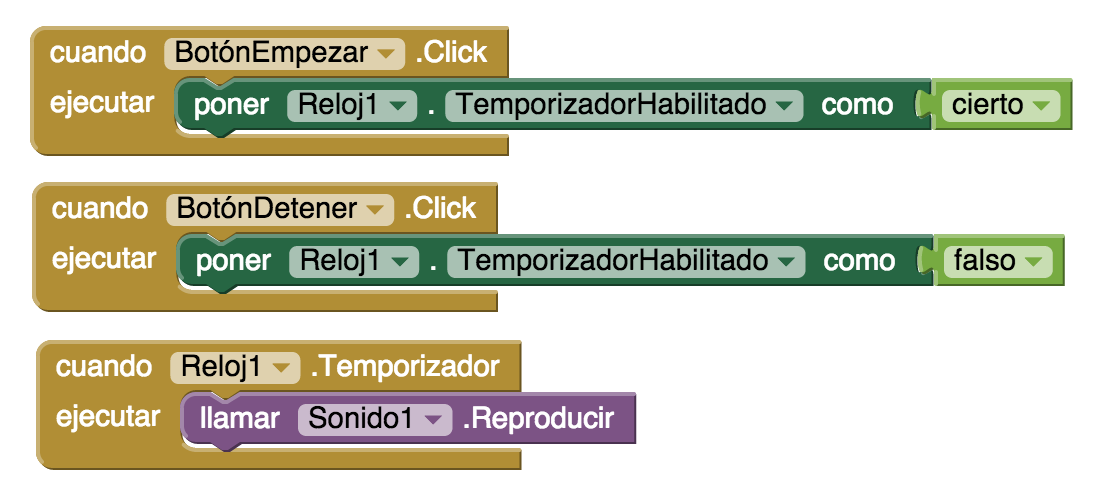
\includegraphics[scale=0.5]{Clock4}
\caption{Cambiar la propiedad \property{TemporizadorHabilitado} del \component{Reloj}.}
\label{fig:Clock4}
\end{figure}

\paragraph{Ejemplo 2: Cuando el usuario habla, la nave empieza a moverse. Cuando el usuario sacude el teléfono, la nave se detiene.}

Para esto necesitas dos componentes adicionales, un
\component{ReconocimientoDeVoz} que puede
reconocer cuando el usuario está hablando, y un \component{Acelerómetro} que detecta
cuando se sacuda el teléfono. El código se muestra en
la~\Cref{fig:Clock5}.

\begin{figure}[H]
\centering
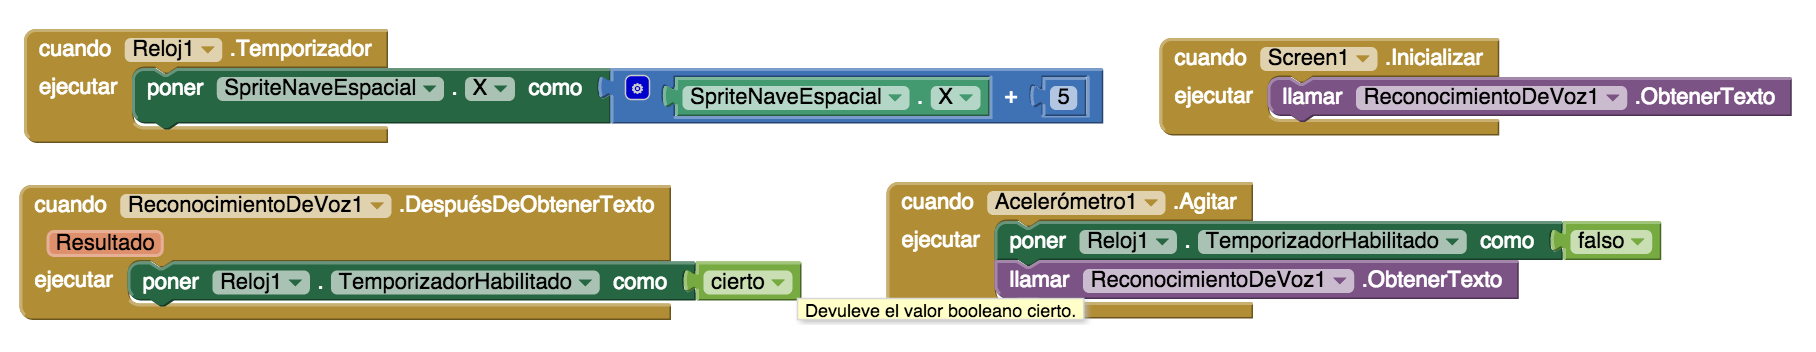
\includegraphics[scale=0.5]{Clock5}
\caption{Moviendo la nave cuando el usuario habla, y deteniéndola
  cuando se agita el dispositivo.}
\label{fig:Clock5}
\end{figure}



El controlador de evento \block{Pantalla.Inicializar} se activa cuando
se inicia la aplicación. El bloque
\block{ReconocimientoDeVoz.ObtenerTexto} abre el sensor de voz para
que espere que el usuario diga algo. Cuando el usuario habla, se
activa el controlador de evento
\block{ReconocimientoDeVoz.SensorVoz.DespuésDeObtenerTexto}. En este
controlador de eventos configurarás la propiedad
\property{Reloj.TemporizadorHabilitado} como verdadera para que el
temporizador se active y así el sprite se empiece a mover. Cuando el
usuario sacude el teléfono, se activa el \component{Acelerómetro}, y
se desactiva el temporizador para que pare el sprite se detenga, y se
vuelva a invocar a \component{ReconocimientoDeVoz.ObtenerTexto}, para
que espere la próxima vez que el usuario hable.

\end{document}
